\section{Analýza problému}
\label{sec:analysis}

Vo všeobecnosti sa za rozvrhový systém považuje softvér, pomocou ktorého
sa vytvárajú rozvrhy. Pri tvorení rozvrhu sa súbor udalostí priraďuje do určitého
počtu časových okamihov, ktoré podliehajú istým súborom obmedzení a pravidiel.
Zvyšovaním počtu udalostí a ohraničení sa zvyšuje aj množstvo kolízií, ktoré je
potrebné minimalizovať či úplne vylúčiť, no zároveň zachovať požadované
obmedzenia a výnimky. Plánovanie a tvorba akademického rozvrhu je výpočtovo
náročný a obvykle zložitý proces. Je to NP úplný problém optimalizácie, ktorý
potrebuje heuristický prístup k nájdeniu riešenia. Hlavnou motiváciou výskumov
v tejto oblasti je minimalizovať celkovú cenu použitých zdrojov pri celom procese
vytvárania rozvrhov.

Samostatnou dôležitou súčasťou riešenia, je nastavenie vhodného zobrazovania
informácií používateľom v systéme a prispôsobiť ho tak, aby bolo používanie čo
najviac intuitívne a prehľadné ako pre rozvrhára, ktorý bude kontrolovať
vygenerovaný rozvrh a ručne upravovať kolízie a udalosti podľa špecifík, tak aj pre
vyučujúcich a študentov, ktorý si budú prezerať svoje rozvrhy. Veľmi dôležitou
funkcionalitou je okrem samotného generovania aj manuálna úprava rozvrhu, ktorá
je z hľadiska časovej náročnosti pre rozvrhára najväčším zdržaním pri tvorbe rozvrhov
(nakoľko automaticky vygenerované rozvrhy nedokážu spoľahlivo nájsť riešenia na
všetky kolízie, osobité požiadavky, výnimky atď).
%------------------------------------------------------------------------------------------------------------------------
%------------------------------------------------------------------------------------------------------------------------
\subsection{Proces tvorby rozvrhu}
\label{subsec:timetabling}

Pri procese tvorby rozvrhu sa jedná o minimalizačný problém, ktorého cieľom je
prehľadať priestor všetkých dostupných možností a nájsť to najlepšie riešenie.
Výstup však musí spĺňať čo najviac vstupných požiadaviek a zároveň zaručiť
splnenie všetkých ohraničení daného prehľadávaného priestoru. Tieto ohraničenia
sa týkajú jednotlivých vstupných elementov ako sú čas (kedy), priestor (kde),
osoba (kto) a iné. \cite{willemen}

\newpage
\begin{figure}[ht]
\centering
\begin{subfigure}{.45\textwidth}
  \centering
  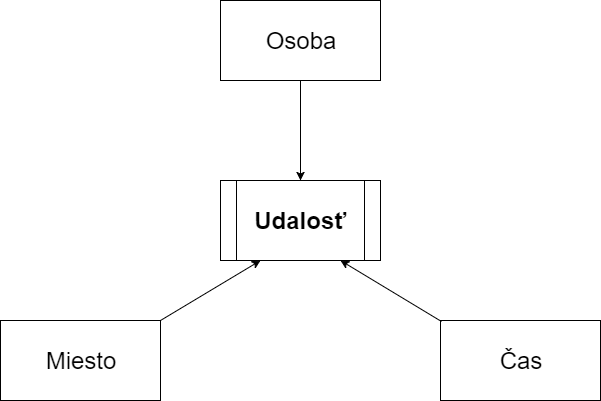
\includegraphics[width=.9\linewidth]{img/koncepty.png}
  \caption{\label{fig:concepts1}}
\end{subfigure}
\begin{subfigure}{.45\textwidth}
  \centering
  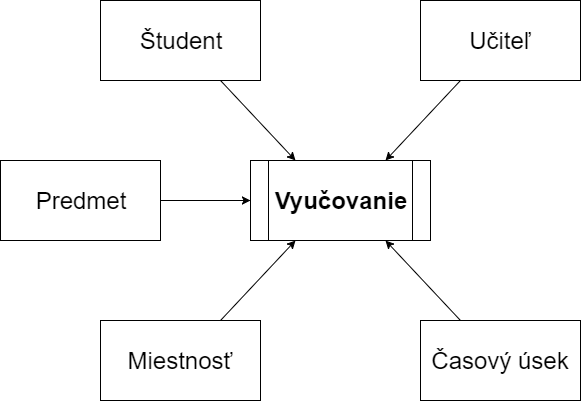
\includegraphics[width=.9\linewidth]{img/koncepty2.png}
  \caption{\label{fig:concepts2}}
\end{subfigure}
\begin{subfigure}{.45\textwidth}
  \centering
  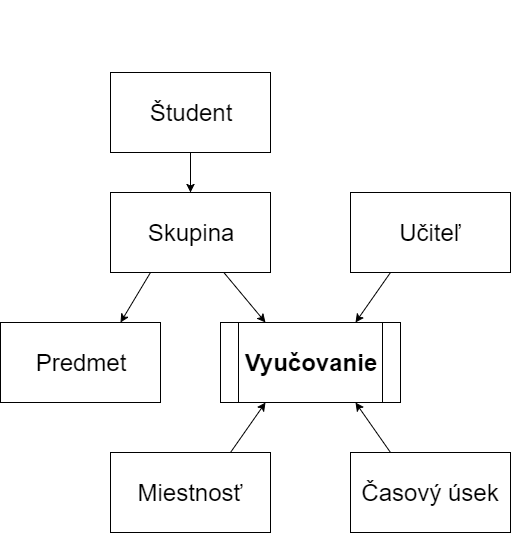
\includegraphics[width=.9\linewidth]{img/koncepty3.png}
  \caption{\label{fig:concepts3}}
\end{subfigure}
\caption{Pojmy a vzťahy medzi nimi používané pri rozvrhoch vo všeobecnosti (a),
pri rozvrhoch na školách (b) a pri rozvrhoch so zaradením študentov do skupín (c) \cite{willemen}}
\label{fig:concepts}
\end{figure}

Ohraničenia sú rozdelené na tvrdé ohraničenia (z angl. Hard Constraints) a mäkké
ohraničenia (z angl. Soft Constraints). Tvrdé ohraničenia nesmú byť porušované
(napr. študent/vyučujúci môže byť v jednom časovom okamihu prítomný iba na
jednom mieste), zatiaľ čo tie mäkké nie je potrebné dodržať, avšak ovplyvňujú
bonitu celého navrhovaného rozvrhu (napr. preferencia časových úsekov, individuálne potreby). \cite{lukac}

Taktiež sa zohľadňujú dáta z predchádzajúcich cyklov a období. Požiadavky sú okrem
doby inicializácie kladené aj počas obdobia semestra, ciže sú dynamické a časom sa môžu
meniť. Jedná sa hlavne o prípady jednorázových udalostí (napr. nahrádzané prednášky
a cvičenia, konferencie, mimovýučbové prednášky). Rozvrh s vyššou bonitou sa všeobecne
považuje za lepší, pretože splnil viac mäkkých ohraničení a je vhodnejší na použitie.
To, či je obmedzenie tvrdé alebo mäkké, sa definuje pri vývoji matematického modelu,
ktorý stojí za problémom plánovania. Na základe toho sa od seba líšia mnohé navrhnuté
implementácie.

Za rozvrh univerzity je spravidla zodpovedný jeden prípadne viacero rozvrhárov
(napr. každý má na starosti rozvrh inej fázy počas roka - výučba / skúškové obdobie).
V dnešnej dobe prevláda zväčša kombinovaná tvorba rozvrhu, kedy sa automaticky
generovaný rozvrh manuálne upravuje rozvrhárom na základe zozbieraných
požiadaviek a určitých obmedzení. Obmedzenia do systému zadávajú samotní
vyučujúci a študenti, prípadne je na túto činnosť pre dané oddelenie priradený
zástupca oddelenia, ktorý má túto činnosť na starosti.

Na nasledujúcom obrázku je znázornený harmonogram akcií pri tvorbe rozvrhu počas semestra:
\begin{figure}[ht]
  \centering
  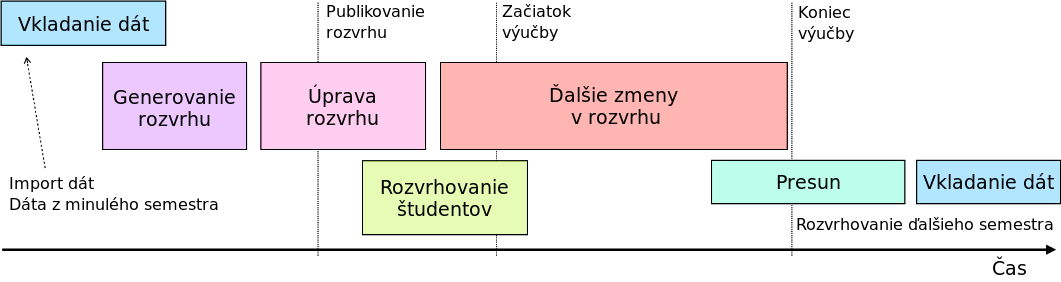
\includegraphics[width=1\columnwidth]{img/course-timetabling.png}
  \caption{\label{fig:course_timetabling} Harmonogram akcií pri tvorbe rozvrhu \cite{unitime_hl}}
\end{figure}

%------------------------------------------------------------------------------------------------------------------------
%------------------------------------------------------------------------------------------------------------------------
\subsection{Existujúce rozvrhové systémy}
\label{subsec:existing_systems}

Rozmanitosť existujúcich rozvrhových systémov zahřňa aj pestrosť v ich ponúkaných funcionalitách
a možnostiach. Ich rozdielnosť najčastejšie spočíva v:
\begin{itemize}
\item podporovanom operačnom systéme,
\item licencii a cene,
\item dizajne používateľského rozhrania,
\item oblasti zamerania (základné školy, stredné školy, univerzity a ďalšie),
\item spôsobe tvorenia rozvrhu (manuálny, automatický, kombinovaný),
\item použitom algoritme generovania rozvrhu,
\item možnostiach úprav zdrojov, udalostí a iných vstupných dát,
\item možnostiach importu a exportu,
\item možnostiach administratívy,
\item zabezpečení.
\end{itemize}

V nasledujúcich podkapitolách si priblížime niektoré z nich z hľadiska poskytovaných funkcionalít
a možností a aj z hľadiska dizajnu používateľského rozhrania.

%------------------------------------------------------------------------------------------------------------------------
\subsubsection{CelCat}
\label{subsubsec:celcat}

CELCAT Timetabler\footnote{\url{ https://www.celcat.com/}} poskytuje integrovaný prístup k časovému
rozvrhovaniu a rezervácii miestností, pričom sa snaží o čo najlepšie využitie zdrojov, priestoru a času.
Jednotný prístup k správe dát umožňuje časomeračom a priestorovým rezervátorom v rámci celej univerzity
s cieľom získať prístup k jedinému, jasnému a koherentnému zdroju informácií o rozvrhovom poriadku.

V CELCAT sú rozvrhy zostrojené ako mriežky, kde sú dni rozdelené na časové bloky, ktoré sú označované
ako obdobia. Udalosti sa vytvárajú v časovej mriežke rozvrhu, ak je jeden alebo viac zdrojov
(napr. zamestnanci, miestnosti, študenti atď.), ktoré sa majú uskutočniť počas jedného alebo viacerých období.

Prístup k CELCAT je zabezpečený prostredníctvom úloh špecifických pre jednotlivé oddelenia. Používatelia majú
zvyčajne prístup k zdrojom a rozvrhom, ktoré sú priamo spojené s ich oddelením. Za výnimočných okolností
môžu používatelia mať prístup k zdrojom, ktoré nie sú okamžite spojené s ich oddelením, ak to predtým
schválili všetky zainteresované oddelenia a udelili mu povolenie \cite{celcat}.

Existujú tri typy používateľov CELCAT:
\begin{itemize}
\item Hlavný rozvrhár celého oddelenia
\item Osoba rezervujúca miestnosti
\item Prezerajúci používateľ (z angl. Read-only user)
\end{itemize}

Všetci používatelia majú prístup len na čítanie ku všetkým zdrojom a rozvrhom, ktoré sú v rámci CELCAT-u.
S cieľom zaistiť bezpečnosť údajov sa používateľské účty vytvárajú len pre pracovníkov, pre ktorých je prístup
k systému CELCAT žiadaný a nevyhnutný.

Dáta sa do systému dajú buď importovať alebo vytvárať ručne. Medzi najhlavnejšie možnosti systému patria:
\begin{itemize}
\item Vytvorenie nového / Otvorenie existujúceho rozvrhu
\item Tlač / zdieľanie rozvrhu / automatické zverejnenie rozvrhu
\item Možnosť spravovania zdrojov
\item Možnosť spravovania udalostí
\item Klasifikácia zdrojov a udalostí
\item Pokročilé funkcie konfigurácie (dĺžka vyučovacích hodín, individuálne podujatia a ďalšie)
\item Konfigurácia miestností (počet sedadiel, vybavenie)
\item Náhľad kalendára udalostí
\item Detekcia kolízií a rôzne úrovne ich riešenia
\item Poradca dostupných zdrojov pre udalosť
\item Podpora štandardných a externých štúdií
\item Štatistiky
\end{itemize}

V prípade systému CELCAT treba spomenúť, že sa jedná o komerčný softvér. Rozhranie je už pomerne zastaralé,
s čím úzko súvisí aj celý používateľský zážitok pri používaní systému. Niektoré bežné príkazy nie sú ľahko prístupné
a vyžadujú si veľa klikov. Ďalším negatívom je fakt, že systém podporuje iba prácu na 4 oknách súčasne.

Podrobnejšie informácie o možnostiach celého systému sú dostupné v dokumente používateľskej príručky
CELCAT\footnote{\url{http://www3.imperial.ac.uk/pls/portallive/docs/1/10225698.PDF}}.

\newpage
\begin{figure}[ht]
  \centering
  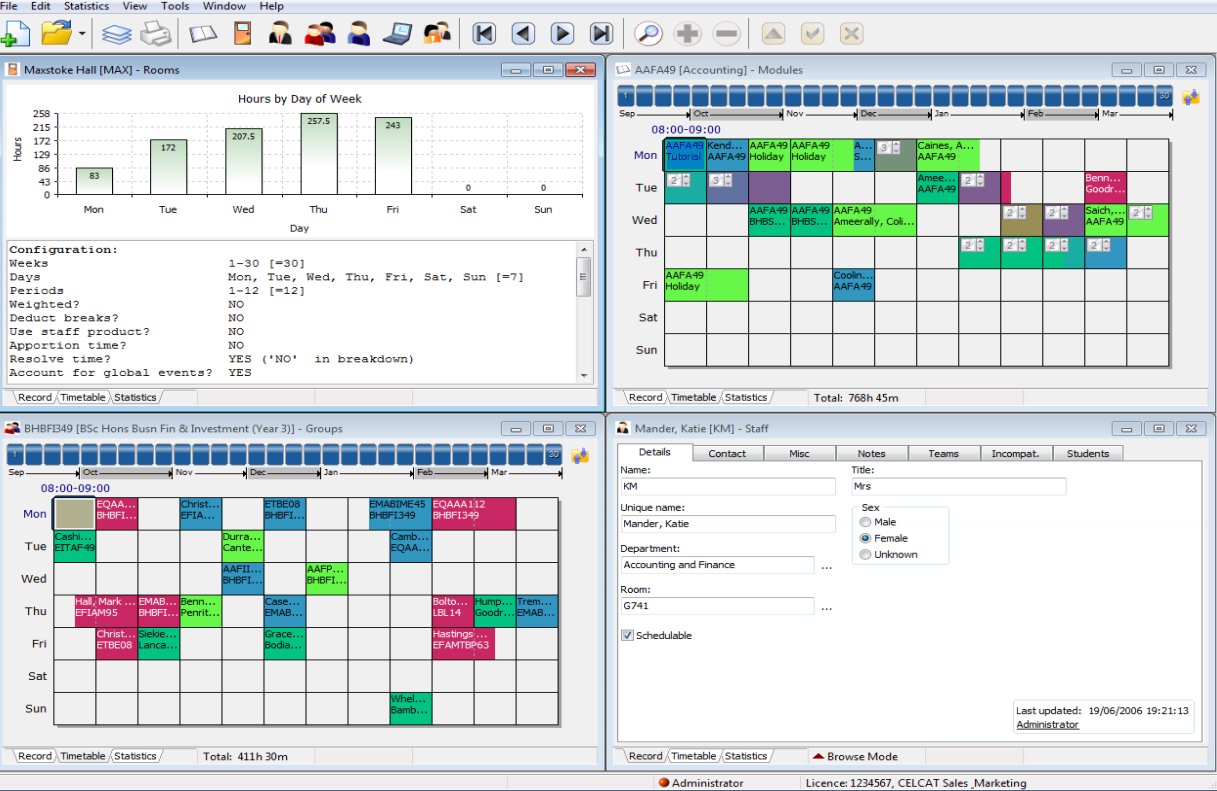
\includegraphics[width=0.71\columnwidth]{img/celcat.jpg}
  \caption{\label{fig:celcat_gui} Náhľad používateľského rozhrania systému CELCAT \cite{celcat}}
\end{figure}

\begin{figure}[ht]
  \centering
  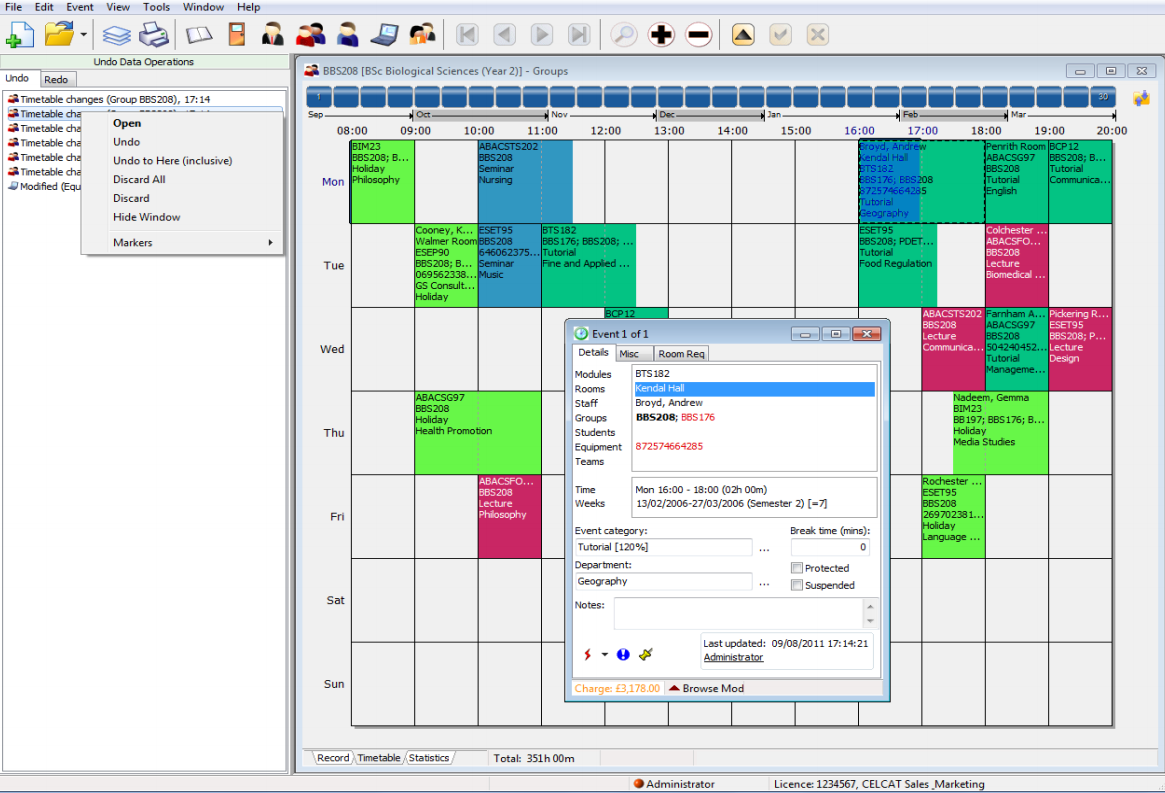
\includegraphics[width=0.71\columnwidth]{img/celcat2.jpg}
  \caption{\label{fig:celcat2_gui} Náhľad kalendára udalostí systému CELCAT \cite{celcat}}
\end{figure}

%------------------------------------------------------------------------------------------------------------------------
\subsubsection{aSc TimeTables}
\label{subsubsec:asc}

Asc TimeTables\footnote{\url{https://www.asctimetables.com/}} je rozvrhový systém,
ktorý je primárne zameraný na stredné školy, pretože je založený na systéme s 8 obdobiami.
Používateľ zadá dni, predmety, učiteľov a učebne, ktoré sa majú zahrnúť do rozvrhu. Po zadaní
všetkých informácií Asc TimeTables vytvorí výsledný rozvrh, ktorý je založený na nasledujúcich kritériách \cite{asc}:

\begin{itemize}
\item Špecifikácia typu predmetu
\item Použitie pravidla proporcionálneho rozloženia hodín počas celého týždňa
\item Okná učiteľov
\item Špecifikácia maximálneho počtu okien učiteľov
\item Špecifikácia maximálneho počtu okien učiteľov za deň
\item Možnosť generovania nultých hodín
\item Možnosť príchodu učiteľa na druhú lekciu alebo dokonca špecifikovať vyučovací blok manuálne
\item Použitie pravidla pre celé a rozdelené formy vyučovacích hodín
\item Pridelenie hodín do jednotlivých tried
\item Zamknutie hodín v určených pozíciách
\item Stanovenie úrovne komplexnosti generovania rozvrhu
\item Počet kariet na otáznych pozíciach v rozvrhu
\item Vzťahy všetkých kariet
\end{itemize}

Medzi kladné stránky systému patrí to, že má jednoduché ovládanie, nakoľko program používa štandardné MS WindowsTM
rozhranie. Asc TimeTables je navrhnutý pre efektívne zadávanie a kontrolu dát. Okrem svojej jednoduchosti poskytuje
Asc TimeTables aj skvelú dokumentáciu, ktorá obsahuje sekciu pre testovanie. Systému však chýba lepšie zabezpečenie,
modul rozsiahlejšej administrácie a možnosť zadávania vstupov a preferencií od študentov.

Bližšie špecifiká možností tohto systému sú dostupné v oficiálnej dokumentácii\footnote{\url{help.asctimetables.com/pdf/asc_timetables_en_P1.pdf/}}
Asc TimeTables systému.

\newpage
\begin{figure}[ht]
  \centering
  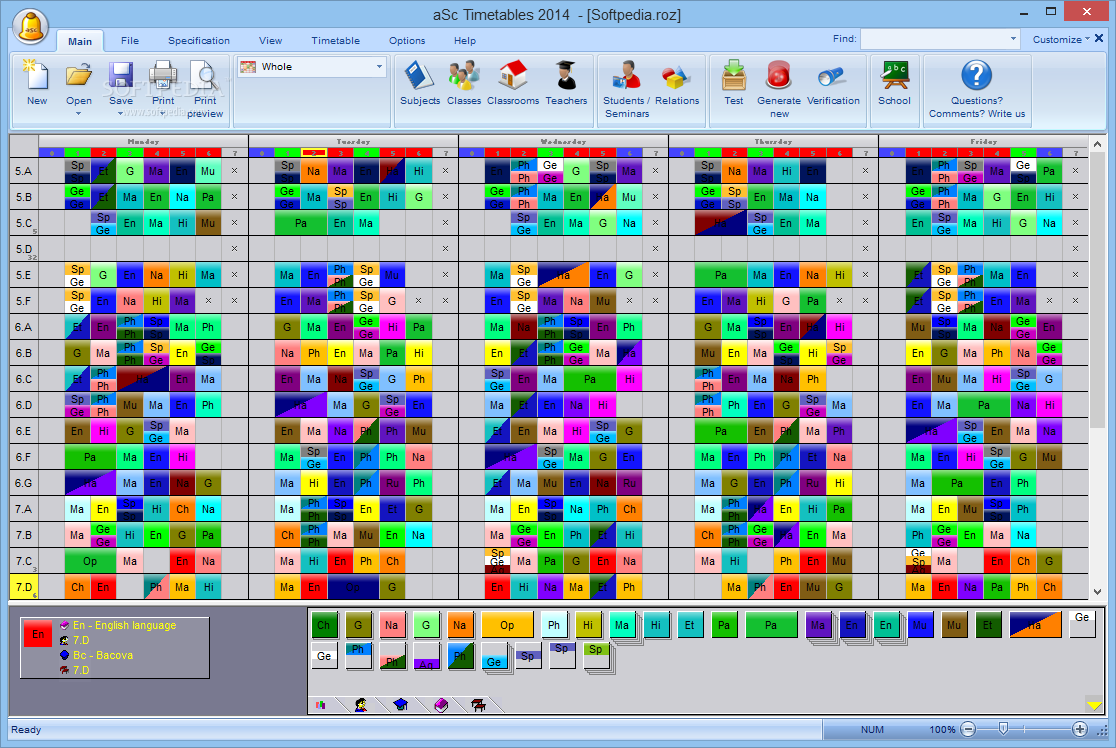
\includegraphics[width=0.71\columnwidth]{img/asc.png}
  \caption{\label{fig:asc_gui} Náhľad používateľského rozhrania systému aSc TimeTables \cite{asc}}
\end{figure}

\begin{figure}[ht]
  \centering
  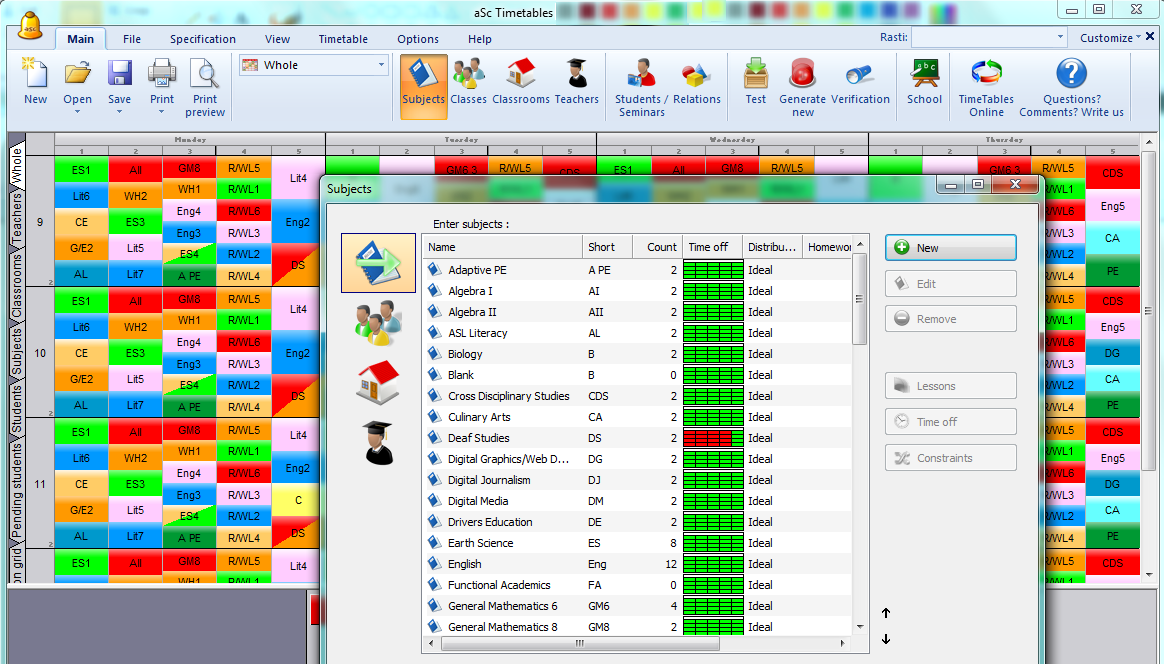
\includegraphics[width=0.71\columnwidth]{img/asc2.png}
  \caption{\label{fig:asc2_gui} Zobrazenie zoznamu predmetov v systéme aSc TimeTables \cite{asc}}
\end{figure}

%------------------------------------------------------------------------------------------------------------------------
\subsubsection{Mimosa}
\label{subsubsec:mimosa}

Rozvrhový systém Mimosa je desktopová aplikácia pre \acrshort{os} Windows, napísaná v jazyku
Borland Delphi, ktorá sa používa na plánovanie udalostí na stredných školách, univerzitách,
ale aj vo firmách. Program používa tabuľky na zadanie informácií od používateľa. Softvér
umožňuje používateľovi zadať kurz, inštruktora a čas, aby zistil, ako vytvoriť rozvrhový plán.
Tvorbu rozvrhu je možné vykonať manuálne, ale v prípade potreby aj automaticky prípadne
 kombinovaným spôsobom. Na prácu s dátami v podobe importu a exportu bola implementovaná
podpora pre formáty CSV, iCalendar, vCalendar. Mimosa má aj vlastný formát dát obdobného názvu \cite{mimosa}.
Systém Mimosa používa svoju vlastnú databázu.

Medzi hlavné výhody systému patria:
\begin{itemize}
\item Rozsiahla funkcionalita
\item Automatická kontrola kolízií
\item Napodobňovanie predchádzajúcich riešení a výber miestností
\item Stromové zobrazenie prehliadania udalostí
\item Funkcia Drag\&Drop
\item Možnosť manuálnej úpravy rozvrhu
\item Kontextová pomoc
\item Podrobná dokumentácia
\end{itemize}

Nevýhodou je podpora iba pre jednu platformu a platená komerčná licencia potrebná na používanie plnej
verzie systému.

\begin{figure}[ht]
  \centering
  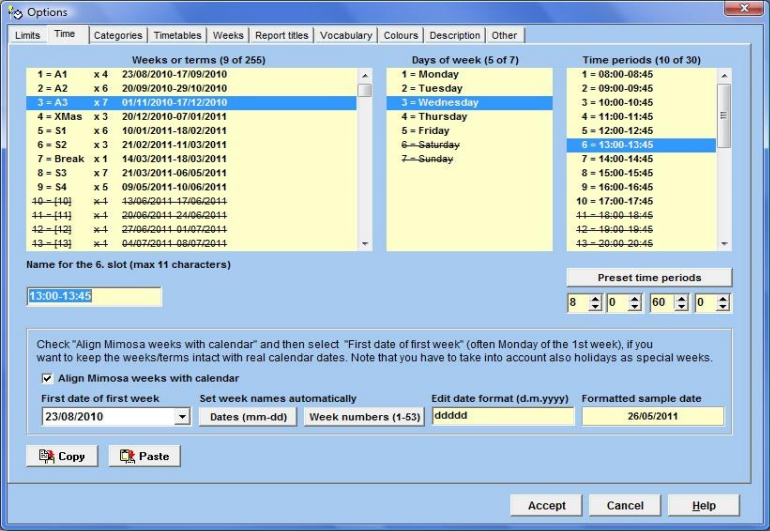
\includegraphics[width=0.71\columnwidth]{img/mimosa_1.png}
  \caption{\label{fig:mimosa1_gui} Zobrazenie nastavení v systéme Mimosa \cite{mimosa}}
\end{figure}

\begin{figure}[ht]
  \centering
  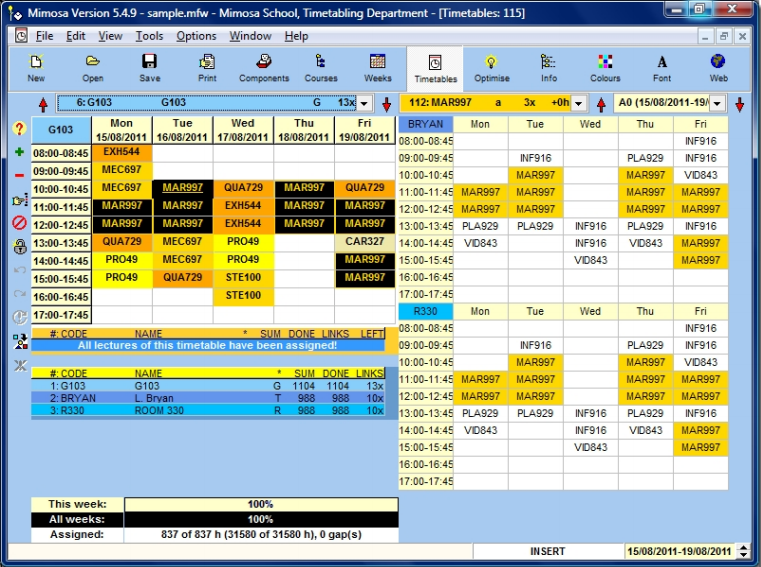
\includegraphics[width=0.71\columnwidth]{img/mimosa_2.png}
  \caption{\label{fig:mimosa2_gui} Zobrazenie rozvrhu v systéme Mimosa \cite{mimosa}}
\end{figure}

%------------------------------------------------------------------------------------------------------------------------
%------------------------------------------------------------------------------------------------------------------------
%------------------------------------------------------------------------------------------------------------------------
\section{Cieľ práce}
\label{sec:goal}

Cieľom našej práce je oboznámiť sa s predchádzajúcimi prácami \cite{knap} a \cite{racak} a na základe existujúcej
implementácie rozšíriť systém o moderné a prehľadné používateľské rozhranie. V predchádzajúcej
práci \cite{racak} bol primárnym cieľom skôr vývoj serverovej časti systému, pričom používateľské rozhranie
bolo iba prototypom napísaným vo funkcionálnom jazyku Elm\footnote{\url{http://elm-lang.org/}}.
My sme sa rozhodli pre vývoj
používateľského rozhrania v novej technológií Angular 5, ktorá v spojení s ďalšími nástrojmi
umožňuje tvoriť moderné aplikácie ako z hľadiska funkcionality, tak aj z hľadiska dizajnu.
%------------------------------------------------------------------------------------------------------------------------
%------------------------------------------------------------------------------------------------------------------------
\subsection{Špecifikácia požiadaviek}
\label{subsec:requirements}

Autori oboch predchádzajúcich prác pomerne jasne špecifikovali požiadavky kladené na celý
rozvrhový systém. Vo všeobecnosti má systém umožňovať:

\begin{itemize}
\item Spravovanie a upravovanie používateľských oprávnení.
\item Pracovanie s dátami, ich import a export dát v spolupráci so systémom AIS
\item Zálohovanie dát a možnosť vytvárania verzií rozvrhov
\item Vkladanie jednotlivých požiadaviek a obmedzení vplývajúcich na tvorbu výsledného rozvrhu
\item Konfigurovanie systémových parametrov ovplyvňujúcich výsledky generátora rozvrhov,
ale aj vzhľad a správanie používateľského rozhrania
\item Automatizované generovanie rozvrhov
\item Manuálne tvorenie rozvrhov a úpravy v nich pomocou intuitívneho prostredia a nástrojov 
Drag\&Drop s funkciou sledovania kolízií
\item Rezervovanie miestností pre nerozvrhové udalosti
\item Navrhovanie vylepšení a iných zmien v rozvrhu jeho vlastnými používateľmi
\end{itemize}

Požiadavky aj naďalej zostávajú rovnaké, avšak naša práca sa zameriava skôr konkrétne
na oblasť používateľského rozhrania a požiadaviek kladených na túto časť systému. 
V tejto oblasti sú kladené ako hlavné tieto požiadavky:

\begin{itemize}
\item Moderný dizajn aplikácie s použitím najnovších technológií
\item Prehľadné a intuitívne používateľské rozhranie
\item Responzívne správanie aplikácie zohľadňujúce rozlíšenie zariadenia
\item Jednoduchá navigácia medzi modulmi systému bez zbytočných preklikov do hĺbky
\end{itemize}
%------------------------------------------------------------------------------------------------------------------------
%------------------------------------------------------------------------------------------------------------------------
\subsection{Tvorba rozvrhov na FEI}
\label{subsec:fei_timetabling}

Na fakulte FEI sa proces
tvorenia rozvrhov rozdeľuje do dvoch fáz osobitne. Jednou fázou je tvorba rozvrhu na
semester a tou druhou je fáza tvorby rozvrhu na skúškové obdobie. Každú z týchto fáz má
na starosti iný rozvrhár. Aktuálny stav procesu tvorenia rozvrhov sme konzultovali s
rozvrhárom Mgr. Dávidom Panczom, PhD. Existujú dva programy na tvorbu rozvrhov,
ktoré majú rozvrhári FEI k dispozícii. Novším z nich je program Roger, ktorý však generuje
horšie výsledky a disponuje obmedzenejšou funkcionalitou manuálnych úprav
vygenerovaných rozvrhov než starší program WinRozvrhy. Preto sa na tvorbu rozvrhov FEI
používa tento starší program. Vo fáze skúškového obdobia sa rozvrhy vytvárajú pomocou
súboru skriptov na import dát a v MS Excel sa manuálne vykonáva čiastočná kontrola kolízií.
Samotný proces začína súborom dát z AIS, ktorý je podkladom pre vstupné parametre pri
generovaní. Tieto dáta obsahujú informácie o zozname miestností, predmetov, učiteľov a
zoznamy daľších elementov a vzťahov medzi nimi. Ďalšími dátami pre rozvrhárov, ktoré
vstupujú do celého procesu, sú jednotlivé požiadavky vyučujúcich. Väčšinu týchto obmedzení
treba zohľadňovať individuálne a zaznamenať ich do systému manuálnymi úpravami. 
Výsledný rozvrh zohľadňuje aj predchádzajúce rozvrhy z daných období. Posledným
krokom procesu je importovanie výsledného rozvrhu do AIS, kde je sprístupnený koncovým
používateľom či už na prezeranie alebo prihlasovanie na rozvrhové akcie v prípade študentov
a taktiež následné zvrejnenie na stránke fakulty.

Zo samotného popisu celého procesu ako aj z konzultácií s rozvrhárom vyplýva, že aktuálny
stav tvorenia rozvrhov je skutočne časovo náročný proces a potreba manuálnych úprav v
neefektívnom rozhraní rozvrhárom komplikuje prácu. Manuálnym zásahom sa však kvôli
individuálnym požiadavkám a obmedzeniam nedá úplne predísť, a preto sa budeme snažiť
celé rozhranie systému orientovať hlavne na jednoduchosť a intuitívnosť používania a
jednotlivé operácie orientovať na časovú úsporu a efektívnosť práce v ňom.
%------------------------------------------------------------------------------------------------------------------------
%------------------------------------------------------------------------------------------------------------------------
%------------------------------------------------------------------------------------------------------------------------
\section{Návrh}
\label{sec:design}

V nasledujúcej kapitole popisujeme návrh nových častí systému ako aj potrebné použité
existujúce časti z predošlých prác riešiacich tento rozvrhový systém. Priblížime si nami navrhovanú
architektúru systému a prejdeme ku samotnému náčrtu dizajnu používateľského rozhrania.
%------------------------------------------------------------------------------------------------------------------------
%------------------------------------------------------------------------------------------------------------------------
\subsection{Architektúra systému}
\label{subsec:architecture}

Medzi požiadavkami kladenými na systém boli jednoduchosť a prehľadnosť používania, moderná
architektúra a dizajn a v neposlednom rade aj platformová nezávislosť. Najvhodnejšou voľbou
pre takto definovaný systém je navrhnúť ho vo forme webovej jednostránkovej aplikácie (z angl. \acrlong{spa}).
Z hľadiska architektúry sa jedná o klient-server aplikačný model.

Klient komunikuje vo formáte \acrshort{json} prostredníctvom \acrshort{rest} \acrshort{api},
ktoré mu poskytuje server cez \acrshort{http}
(resp. \acrshort{https}). Model klientskej časti pokryjeme modernou Redux architektúrou, ktorá je momentálne
na vzostupe a je vhodná pre systémy so zložitejšími a rozsiahlejšími úpravami globálneho stavu aplikácie.

Serverovú časť rozvrhového systému zabezpečuje webová služba poskytujúca \acrshort{rest} \acrshort{api}
a podľa potreby dáta vyberá z alebo ukladá do PostgreSQL databázy. Architektúru serverovej
časti sme sa rozhodli použiť z predchádzajúcej práce \cite{racak}.
%------------------------------------------------------------------------------------------------------------------------
\subsubsection{Jednostránková aplikácia}
\label{subsubsec:spa}

Vývoj webových aplikácií bol vždy významnou súčasťou vývoja softvéru.
V interakcii s komplexnými webovými aplikáciami však bolo veľa obmedzení,
čo spôsobilo, že nie sú tak responzívne ako desktopové aplikácie.

Prvé webové aplikácie boli jednoduché statické stránky vytvorené
iba s \acrshort{html} a \acrshort{css}. Tieto statické stránky boli pomalé, pretože každá
stránka, teda všetky \acrshort{html} a \acrshort{css}, museli byť stiahnuté zo servera vždy,
keď používateľ klikol na odkaz. Všetko sa zmenilo s príchodom \acrshort{ajax}, a teda
asynchrónneho \acrlong{js}-u a \acrshort{xml}. \acrshort{ajax} je súbor techník, ktoré umožnili web
aplikácii rýchle inkrementálne aktualizácie používateľského rozhrania bez
opätovného načítania celej stránky prehliadača. V porovnaní s čisto statickými
webovými stránkami, ktoré si používateľ musel stiahnuť pri každom kliknutí na odkaz,
boli webové stránky používajúce \acrshort{ajax} mnohokrát rýchlejšie.

Medzičasom sa vyvíjali a vylepšovali nové verzie tradičných technológií používaných
na vývoj webových aplikácií ako \acrshort{html}, \acrshort{css} a \acrshort{js}, čo umožňovalo vytvoriť
novú generáciu flexibilných webových jednostránkových aplikácií. Tento nový typ webovej
aplikácie je z hľadiska interaktivity porovnateľný s desktopovými aplikáciami, a zároveň
nevyžaduje žiadne ďalšie doplnky na fungovanie. Jediná požiadavka, ktorá by mala byť
ideálne splnená, je práca s najnovšiou verziou webového prehliadača. Toto môže byť
považované za nevýhodu týchto aplikácií, pretože podpora \acrlong{js}-u je neustále
rozsiahlym problémom. Stále existuje veľa používateľov, ktorí nie vždy aktualizujú svoje
webové prehliadače na najnovšiu verziu alebo dokonca úmyselne vypnú \acrshort{js}
z bezpečnostných dôvodov alebo z dôvodu ochrany osobných údajov.

Jednostránkové aplikácie pokračovali v raste a objavovala sa potreba lepšej štruktúry
týchto aplikácií. Vývojári začali vytvárať komponenty na lepšiu organizáciu kódu aplikácií.
Jedna z prvých knižníc na báze komponentov bola React\footnote{\url{https://reactjs.org/}}, ktorú vytvoril Facebook.
Keďže React bol len knižnicou na vykresľovanie dát, vznikala bočná potreba spravovania
údajov vo veľkých aplikáciách. Pre tento problém s riadením údajov bol predstavený
architektonický vzor nazývaný Flux. Po jeho uvoľnení začali mnohé vývojárske tímy
realizovať svoje vlastné implementácie Flux-u.

%------------------------------------------------------------------------------------------------------------------------
\subsubsection{Redux}
\label{subsubsec:redux}

Existuje veľa rôznych architektonických vzorov, ktoré sa dajú použiť pri vývoji
webových aplikácií. \acrshort{mvc} (\acrlong{mvc}) je veľmi populárny, široko
podporovaný vzor, používaný už niekoľko desiatok rokov.
Model uchováva údaje potrebné pre aplikáciu. Zobrazenie je nevyhnutné na zobrazenie
dát používateľovi. Riadiaci systém funguje ako lepidlo medzi modelmi a zobrazeniami.
Vyžaduje údaje z modelu a počúva na udalosť v zobrazení \cite{maccaw}.
Treba poznamenať, že existuje veľa \acrshort{mvc} podobných architektúr, \acrshort{mvp} (\acrlong{mvp}),
\acrshort{mvvm} (\acrlong{mvvm}) alebo \acrshort{hmvc} (\acrlong{hmvc}),
ktoré sú buď variáciou alebo odvodením vzoru \acrshort{mvc}.

\newpage
Najjednoduchšia verzia \acrshort{mvc} je znázornená na obrázku nižšie:
\begin{figure}[ht]
  \centering
  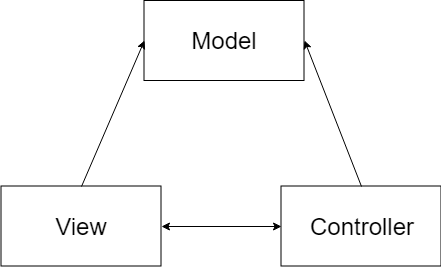
\includegraphics[width=0.6\columnwidth]{img/mvc.png}
  \caption{\label{fig:mvc} Architektúra MVC}
\end{figure}

Manažment stavu aplikácie bol vo frontendových frameworkoch vždy neustálym
problémom. Základná myšlienka mutácie stavov na viacerých úrovniach pri
frontendových frameworkoch robí \acrshort{mvc} prístup neefektívny.
Jeden z hlavných rozdielov medzi Redux\footnote{\url{https://redux.js.org/}}
a \acrshort{mvc} je tok dát. \acrshort{mvc} umožňuje obojsmerný dátový tok, zatiaľ čo Redux
používa jednosmerný dátový tok. Napríklad v \acrshort{mvc} môžu dáta prúdiť z \textit{View}
do \textit{Controller} a naspäť, zatiaľ čo pri Redux-e musí byť zmena vykonaná
prostredníctvom vyvolania akcie.

Stavová mutácia bola zrejmá už v Angular 1 (AngularJS\footnote{\url{ https://angularjs.org/}}),
kde bola logika riadenia stavu aplikácie rozdelená medzi direktívy, kontrolery a službu,
pričom každá úroveň mala svoju vlastnú logiku pre mutáciu stavu. Tým sa segmentovaný
stav celej aplikácie stal náchylný na nekonzistentnosť a takmer nemožný na otestovanie.
Tieto problémy sa stávali čoraz zjavnejšími a ťažšie sa im predcházalo, keďže vývoj
aplikácií napredoval a ich zložitosť časom narastala. Frontendové aplikácie sa začali
stávať čoraz komplexnejšími a reaktívnejšími voči používateľským vstupom. Avšak
čoraz populárnejšie znaky vývoja frontendu, ako napr. dôraz na funkcionálne
programovanie, podporili vznik nového prístupu manažovania stavu aplikácie.

Hlavnou motiváciou pre Redux bola predvídateľnosť stavových mutácií a zníženie
zložitosti spravovania údajov v aplikáciách pomocou jednosmerného toku údajov.
Pretože v systéme Redux toky prechádzajú iba jedným smerom a stav aplikácie
sa nadhádza na jednom mieste, celý systém sa stáva viac predvídateľným.
Redux tiež používa nemeniteľné spravovanie údajov, ktoré spôsobuje menej
vedľajších účinkov v toku dát, čo vedie k jednoduchšiemu programovaniu a ladeniu \cite{piispanen}.

Redux sa skladá z troch hlavných častí.
Prvou časťou sa nazýva úložisko (z angl. Store), v ktorom je
uložený stav a každá časť údajov aplikácie. Je to čistý \acrshort{js} objekt,
ktorý môže byť vytvorený viacerými spôsobmi. Úložisko v Redux-e je nemeniteľné. 
Ďalšou časťou sú akcie (z angl. Actions). Akcie sú taktiež jednoduché \acrshort{js} objekty, ktoré
zabezpečujú informáciu o tom, čo sa má stať, ale neuvádzajú spôsob ani samotnú
logiku, ako by sa to malo robiť. Akcie obsahujú údaje, ktoré sa odosielajú do úložiska.
Poslednou časťou sú reduktory (z angl. Reducers), ktoré spájajú úložisko a akcie.
Reduktory obsahujú logiku aplikácie a sú to jednoduché čisté funkcie (z angl. Pure functions), ktoré
robia zmeny v úložisku. Reduktory nemenia existujúce údaje, ale vždy vrátia úplne nové údaje.

Redux teda sleduje tri základné princípy \cite{redux}:
\begin{itemize}
\item Jednosmerný tok údajov.
\item Stav celej aplikácie je uložený v jedinom nemeniteľnom stavovom strome.
Jediný spôsob, ako zmeniť stav, je vyvolať akciu.
\item Zmeny v úložisku sa vykonávajú pomocou čistých funkcií (z angl. Pure functions).
To znamená, že nemenia pôvodný stav, ale vracajú nové stavové objekty.
\end{itemize}

Pri dodržaní týchto zásad môžeme dosiahnuť predvídateľné a reprodukovateľné
správanie v aplikácii.

Nasledujúci obrázok popisuje tok dát v architektúre Redux:
\begin{figure}[ht]
  \centering
  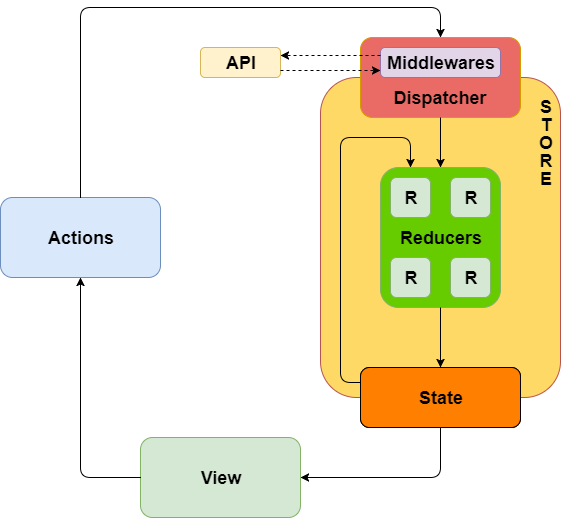
\includegraphics[width=0.8\columnwidth]{img/redux_flow.png}
  \caption{\label{fig:redux_flow} Redux - tok dát v procese \cite{ngredux}}
\end{figure}
\newpage

Napriek tomu, že Redux vznikol prostredníctvom komunity React\footnote{\url{https://reactjs.org/}},
knižnice tretích strán ako napríklad ngrx/store\footnote{\url{https://github.com/ngrx/store}}
a rozšírenia ako \acrshort{rxjs}\footnote{\url{http://reactivex.io/rxjs/}}, urobili z Redux-u
rovnako vhodný koncept na použitie v aplikáciách Angular. Redux je jednou z mnohých
implementácií Flux-u\footnote{\url{https://facebook.github.io/flux/}}.
Populárny sa stal najmä pre širokú komunitu a dobrú dokumentáciu.

Redux pomáha udržať kód ľahšie čitateľný, udržiavateľný a rozrastajúci. Redux je tiež
škálovateľný. Existuje jednoduchý a jasný spôsob, ako rozšíriť aplikáciu, ktorá používa
Redux. Napríklad akcie (z angl. Actions) môžu byť uložené v samostatnom súbore, takže nie sú roztrúsené
naprieč celým kódom aplikácie. Tiež reduktory (z angl. Reducers) môžu byť uložené na jednom mieste
pre jasnú štruktúru. Keď sa v Redux-e pridáva nová funkcia, musí byť vytvorená
akcia. Potom musí byť do reduktora pridaná funkcia, ktorá vykoná skutočnú zmenu
v úložisku (z angl. Store). Redux má aj svoje nevýhody, pretože je spojený s písaním väčšieho počtu
opakovaného kódu ako pri štandardných architektúrach. Taktiež je relatívne ťažké migrovať
existujúci projekt na používanie systému Redux, pretože používa radikálne odlišný prístup
na riadenie stavu aplikácie a toku údajov.

%------------------------------------------------------------------------------------------------------------------------
\subsubsection{REST}
\label{subsubsec:rest}

Reprezentatívny stavový  prevod (\acrshort{rest}) je architektonický štýl, ktorý definuje súbor
obmedzení a vlastností založených na protokole \acrshort{http}. Webové služby, ktoré zodpovedajú
architektonickému štýlu \acrshort{rest} alebo RESTful webové služby, zabezpečujú interoperabilitu
medzi počítačovými systémami na internete. Webové služby kompatibilné s \acrshort{rest} umožňujú
žiadajúcim systémom prístup a manipuláciu s textovými reprezentáciami webových zdrojov
pomocou jednotnej a vopred definovanej množiny bezstavových operácií. Iné druhy webových
služieb, ako sú webové služby \acrshort{soap} (\acrlong{soap}), vystavujú svoje vlastné
sady operácií, čim sa stávajú robustnejšie. \acrshort{rest} využíva menšiu šírku pásma, čo ho robí
vhodnejším na internetové použitie v porovnaní s technológiou \acrshort{soap}.

Vo webovej službe RESTful, môžu byť odpovede na dotazy kladené na \acrshort{uri} zdrojov vo formáte
\acrshort{xml}, \acrshort{html}, \acrshort{json} alebo v inom formáte. Odpoveď môže potvrdiť, že došlo k nejakej zmene
uloženého prostriedku a odpoveď môže poskytnúť hypertextové odkazy na iné súvisiace zdroje
alebo zbierky zdrojov. Pri komunikácii najčastejšie prostredníctvom \acrshort{http} protokolu sú k dispozícii
operácie GET, POST, PUT, DELETE a ďalšie preddefinované metódy \acrshort{crud} \acrshort{http}.

Pomocou bezstavových protokolov a štandardných operácií sa systémy \acrshort{rest} zameriavajú na
rýchly výkon, spoľahlivosť a schopnosť rozširovania tým, že opätovne používajú komponenty,
ktoré je možné spravovať a aktualizovať bez toho, aby to ovplyvnilo systém ako celok,
a to aj počas jeho prevádzky \cite{fielding}.

%------------------------------------------------------------------------------------------------------------------------
\subsubsection{Autentifikácia}
\label{subsubsec:authentification}

Autentifikácia je proces rozpoznávania identity používateľa. Je to mechanizmus, ktorý
spája prichádzajúcu požiadavku so súborom identifikačných poverení. Poskytnuté poverenia
sa porovnávajú s údajmi o používateľských oprávneniach uložených v databáze v lokálnom
operačnom systéme alebo v autentizačnom serveri. Proces overovania vždy beží na začiatku
spustenia aplikácie ešte predtým, ako dôjde ku kontrole a povereniu oprávnení a skôr, než budú
povolené ďalšie operácie v aplikácii. Rôzne systémy môžu vyžadovať rôzne typy poverení
na zistenie totožnosti používateľa. Identifikačné poverenie často nadobúda formu hesla, ktoré je
tajné a známe iba jednotlivcovi a systému.

Proces pozostáva z jednoduchých krokov:
\begin{itemize}
\item Používateľ sa pokúša pripojiť k webovým službám.
\item Webové služby požiadali používateľa o poverenie (informácie o totožnosti).
\item Používateľ poskytuje poverenia.
\item Webové služby overujú totožnosť používateľa overovaním zadaných poverení a zodpovedajúcim
spôsobom odpovedajú.
\end{itemize}

Proces overovania je možné opísať v dvoch odlišných fázach - identifikácia a skutočná autentifikácia.
Identifikačná fáza poskytuje používateľovi identitu s bezpečnostným systémom. Táto identita
je poskytovaná vo forme ID používateľa. Bezpečnostný systém vyhľadá všetky abstraktné
objekty, ktoré pozná, a nájde konkrétnu, ktorú aktuálny používateľ momentálne používa.
Akonáhle sa to stane, používateľ bol identifikovaný. Skutočnosť, ktorú používateľ tvrdí, však
nevyhnutne nemusí byť pravdivá. Skutočný používateľ môže byť priradený k inému abstraktnému
používateľskému objektu v systéme, a preto mu musia byť udelené práva a povolenia a používateľ
musí systému poskytnúť dôkazy preukazujúce jeho totožnosť. Proces určenia nároku na totožnosť
používateľa prostredníctvom kontroly dôkazov poskytnutých používateľmi sa nazýva autentifikácia
a dôkaz, ktorý poskytuje používateľ počas procesu autentifikácie, sa nazýva identifikačné poverenie.

\acrshort{rest} framework poskytuje niekoľko schém autentifikácie a tiež umožňuje implementovať vlastné
schémy. Schémy overovania sú vždy definované ako zoznam tried. \acrshort{rest} sa pokúsi autentifikovať
s každou triedou v zozname a nastaví \textit{request.user} a \textit{request.auth} pomocou
návratovej hodnoty prvej úspešne overenej triedy. Ak sa žiadna trieda neoverí, \textit{request.user}
bude nastavené na inštanciu \textit{django.contrib.auth.models.AnonymousUser}
a \textit{request.auth} bude nastavené na \textit{None}.

Hodnotu \textit{request.user} a \textit{request.auth} pre neoverené požiadavky je možné upraviť
pomocou nastavení \textit{UNAUTHENTICATED\char`_USER} a \textit{UNAUTHENTICATED\char`_TOKEN}.

Nižšie si popíšeme niekoľko bežných autentifikačných schém používaných pri \acrshort{rest} webových službách.

\vskip 0.5cm
\textbf{Basic Authentication} schéma používa základnú autentifikáciu \acrshort{http}, podpísanú používateľským
menom a heslom v dotaze. Je to najjednoduchší spôsob implementácie overovania. V tejto schéme
sa informácie o používateľskej totožnosti, tj poverenia, odosielajú v zakódovanom formáte \textit{base64}.
Získaná zakódovaná hodnota \textit{base64} sa odošle pomocou \acrshort{http} hlavičky \textit{Authorization} \cite{rfc7617}.
Ak sa úspešne overí, \textit{Basic Authentication} poskytuje nasledujúce poverenia.
\begin{itemize}
\item \textit{request.user} bude Django inštancia typu \textit{User}.
\item \textit{request.auth} bude \textit{None}.
\end{itemize}

Neoverené odpovede, ktorým sa odmietne povolenie, spôsobia neoprávnenú odpoveď
\textit{HTTP 401 Unauthorized} s príslušnou hlavičkou \textit{WWW-Authenticate}.

Problém s touto schémou overovania je, že používateľské meno a heslo sú zakódované a nie šifrované,
čiže sa dajú ľahko dekódovať. V dôsledku tohto problému by nemala byť základná schéma overenia
implementovaná tam, kde komunikácia prebieha cez \acrshort{http} a nie cez \acrshort{https}.
Základné overenie je vo všeobecnosti vhodné iba na testovanie.

Odosielané poverenia pri schéme \textit{Basic Authentication} môžu napríklad vyzerať nasledovne:
\begin{figure}[ht]
  \centering
  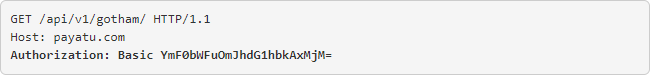
\includegraphics[width=1\columnwidth]{img/auth_basic.png}
  \caption{\label{fig:auth_basic} Príklad poverenia pri schéme Basic Authentication \cite{payatu}}
\end{figure}


\textbf{HMAC Authentication} schéma, pri ktorej namiesto odosielania hesla v zakódovanej podobe
posiela klient hash hodnotu hesla s inými informáciami. Iné informácie vo všeobecnosti pozostávajú
zo slovies (operácií) \acrshort{http}, z \acrshort{url}, časovej pečiatky, hashu v tele správy alebo náhodného čísla.
Vhodným riešením je použiť hodnotu hash správy tela pri konštrukcii HMAC hashu, pretože zabezpečí
integritu odosielaných údajov.

Ak napríklad používateľ \textit{batman} pristupuje k prostriedku \textit{gotham}, potom výpočet HMAC môže vyzerať
nasledovne:
\begin{figure}[ht]
  \centering
  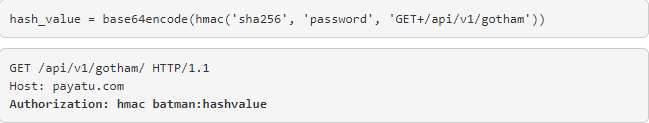
\includegraphics[width=1\columnwidth]{img/auth_hmac.png}
  \caption{\label{fig:auth_hmac} Príklad poverenia pri schéme HMAC \cite{payatu}}
\end{figure}


\textbf{Token Authentication} schéma používa jednoduchú schému \textit{Authentication \acrshort{http}} založenú na tokenoch.
Autentifikácia prostredníctvom tokenu je vhodná pre nastavenia klient-server, ako sú natívni desktopoví
a mobilní klienti. Reťazec je podpísaný serverom a klient ho získa po požiadaní o jeho vytvorenie ako odpoveď.
Sever si však nemusí nič pamätať a všetky potrebné informácie sú uložené a kryptograficky zakódované v tokene.
Jednou z vlastností tokenu je aj jeho ohraničená platnosť.

Ak chceme použiť schému \textit{Token Authentication}, musíme nakonfigurovať triedy autentifikácie tak,
aby zahŕňali \textit{TokenAuthentication} a navyše obsahovali \\
\textit{rest\char`_framework.authtoken} v nastavení \textit{INSTALLED\char`_APPS}.

Odosielané poverenia pei schéme Token Authentication môžu napríklad vyzerať nasledovne:
\begin{figure}[ht]
  \centering
  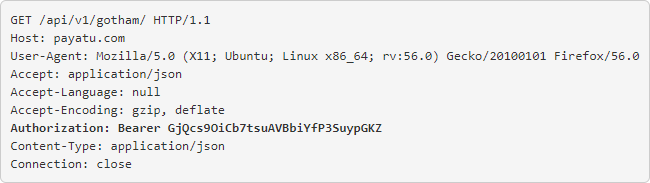
\includegraphics[width=1\columnwidth]{img/auth_token.png}
  \caption{\label{fig:auth_token} Príklad poverenia pri schéme Token Authentication \cite{payatu}}
\end{figure}

V našom systéme je na \acrshort{rest} \acrshort{api} autentifikáciu používaná schéma \textit{Token Authentication}.
Tá udržiava bezstavovost servera a je vhodná pre nastavenia klient-server pre desktopových
aj mobilných klienov. Autor predchádzajúcej práce \cite{racak} sa rozhodol konkrétne pre štandard
\acrshort{jwt} (\acrlong{jwt}).

%------------------------------------------------------------------------------------------------------------------------
\subsubsection{JSON Web Token}
\label{subsubsec:json_web_token}

\acrlong{jwt} je otvorený štandard založený na formáte \acrshort{json} pre vytváranie prístupových
tokenov, ktoré obsahujú istý počet tvrdení. Napríklad server by mohol vygenerovať token, ktorý
obsahuje tvrdenie \textit{``prihlásený ako admin''} a poskytne ho klientovi. Klient by potom mohol
použiť token, aby dokázal, že je prihlásený ako admin. Tokeny sú podpísané súkromným kľúčom
jednej strany (zvyčajne serverom), takže obidve strany (ostatné, ktoré už sú vhodným
a dôveryhodným spôsobom v držbe príslušného verejného kľúča) dokážu overiť, že token je
legitímny. Tokeny sú navrhnuté tak, aby boli kompaktné, bezpečné pre adresy \acrshort{url} a použiteľné
najmä v kontexte jednotného prihlásenia webového prehliadača (\acrshort{sso}). Tvrdenia \acrshort{jwt} sa môžu 
zvyčajne používať na odovzdávanie totožnosti overených používateľov medzi poskytovateľom
totožnosti a poskytovateľom služieb alebo akýchkoľvek iných typov tvrdení, vyžadovaných
obchodnými procesmi. \acrshort{jwt} majú zvyčajne tri časti a to hlavičku, užitočné dáta a podpis \cite{jwt_io}.

\vskip 0.5cm
\textbf{Hlavička} identifikuje, ktorý algoritmus sa používa na generovanie podpisu, a môže
vyzerať takto \cite{rfc7519}:

\lstset{
    string=[s]{"}{"},
    stringstyle=\color{blue},
    comment=[l]{:},
    commentstyle=\color{black},
    basicstyle=\ttfamily
}

\begin{lstlisting}
{
  "alg": "HS256",
  "typ": "JWT"
}
\end{lstlisting}
HS256 označuje, že tento token je podpísaný pomocou \textit{HMAC-SHA256}.

\vskip 0.5cm
\textbf{Užitočné dáta} obsahujú tvrdenia a metadáta. Existujú tri typy tvrdení a to
registrované, verejné a súkromné tvrdenia.

\begin{itemize}
\item Registrované tvrdenia: Ide o súbor odporúčaných preddefinovaných tvrdení, ktoré nie sú povinné.
Sem patria napríklad tvrdenia iss (vydavateľ), exp (čas expirácie), sub (predmet), aud (publikum) a ďalšie.
\item Verejné tvrdenia: Môžu byť ľubovolne definované používateľmi JWT. Aby sa však zabránilo kolíziám,
mali by byť definované v registri \acrshort{iana} \acrshort{json} alebo definované ako \acrshort{uri},
ktoré obsahuje menný priestor odolný voči kolíziam.
\item Súkromné tvrdenia: Ide o vlastné tvrdenia vytvorené na zdieľanie informácií medzi stranami,
ktoré súhlasia s ich použitím a nepatria medzi registrované ani verejné tvrdenia.
\end{itemize}

Objekt užitočných dát môže vyzerať nasledovne:
\begin{lstlisting}
{
  "sub": "1234567890",
  "name": "John Doe",
  "admin": true
}
\end{lstlisting}

\vskip 0.5cm
\textbf{Podpis} je vypočítaný pomocou algoritmu deklarovaného v hlavičke, ktorý spojí tajomstvo
so zakódovanou hlavičkou a užitočnými dátami, ktoré sú oddelené bodkou.
Ak napríklad chceme použiť algoritmus \textit{HMAC SHA256}, podpis sa vytvorí nasledujúcim spôsobom:

  \begin{verbatim}
  HMACSHA256(
    base64UrlEncode(hlavička) + "." + base64UrlEncode(užitočné dáta),
    tajomstvo)
  \end{verbatim}

Podpis sa používa na overenie toho, že správa nebola počas prenosu zmenená a v prípade tokenov
podpísaných so súkromným kľúčom môže tiež overiť, že odosielateľ JWT je ten, kým tvrdí že je.

Nasledujúci text zobrazuje \acrshort{jwt}, ktorý má zakódovanú predchádzajúcu hlavičku a užitočné dáta
a je podpísaný s tajomstvom.

\begin{verbatim}
eyJhbGciOiJIUzI1NiIsInR5cCI6IkpXVCJ9.
eyJzdWIiOiIxMjM0NTY3ODkwIiwibmFtZSI6IkpvaG4gRG9lIiwiYWRtaW4iOnRydWV9.
TJVA95OrM7E2cBab30RMHrHDcEfxjoYZgeFONFh7HgQ
\end{verbatim}

Bližšie informácie o konkrétnej implementácii \acrshort{jwt} v našom systéme sú popísané
v predchádzajúcej diplomovej práci \cite{racak}.
%------------------------------------------------------------------------------------------------------------------------
%------------------------------------------------------------------------------------------------------------------------
\subsection{Návrh používateľského rozhrania}
\label{subsec:gui}

Najdôležitejšou časťou používateľského rozhrania je kalendár udalostí. Do kalendára
sa dajú vkladať nové udalosti, upravovať a prípadne mazať už existujúce. Kalendár
podporuje Drag\&Drop funkcionalitu, pomocou ktorej sa dajú jednotlivé udalosti v kalendári
presúvať na iné miesta časovej mriežky a takisto podporuje funkcionalitu rozširovania časového
rozsahu existujúcej udalosti ťahaním jej okrajov. Klient umožňuje zobrazenie časovej mriežky
z viacerých náhľadov, a to na dňovej, týždňovej a mesačnej úrovni. Inšpirovali sme sa riešeniami
z vyššie popísaných existujúcich rozvrhových systémov \ref{subsec:existing_systems}
a z hľadiska dizajnu podľa Kalendáru Google\footnote{\url{https://calendar.google.com}}
a aplikácie Vonigo\footnote{\url{https://dribbble.com/shots/1458422-Vonigo-Schedule/attachments/216307}}.
Návrh rozhrania pre kalendár udalostí je načrtnutý na obrázku \ref{fig:gui_design} nižšie.

\newpage
\begin{figure}[ht]
  \centering
  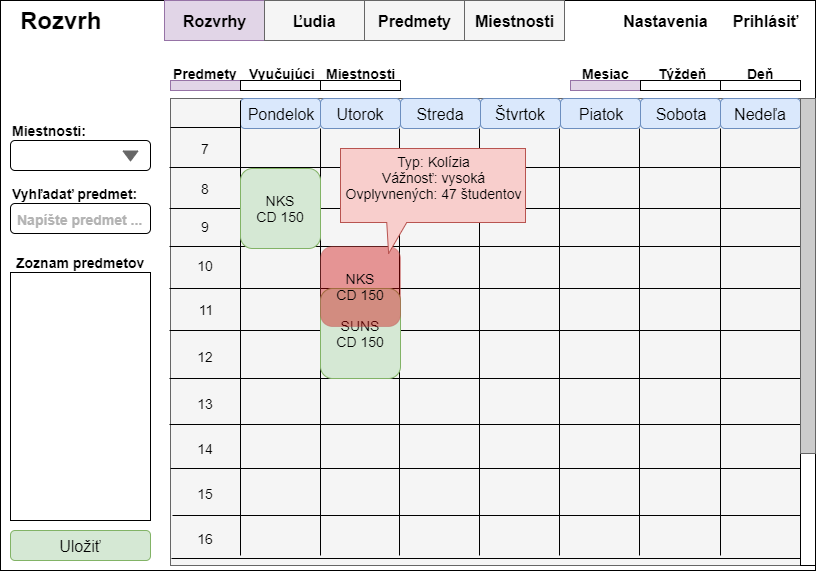
\includegraphics[width=1\columnwidth]{img/screen_view_schedule.png}
  \caption{\label{fig:gui_design}Návrh rozhrania pre kalenár udalostí}
\end{figure}

Na základe špecifikovaných požiadaviek \ref{subsec:requirements} je aplikácia prehľadná
a práca s ňou nevyžaduje zbytočné prekliky na uskutočnenie jednoduchých operácií. 
Používateľské rozhranie je schopné prispôsobiť sa viacerým druhom zariadení a jeho správanie
je plne responzívne zohľadňujúc rozlíšenie zariadenia a možnosti voľného priestoru na obrazovke.
Menu celej aplikácie a navigácia medzi modulmi je vedená v duchu jednoduchosti na báze
dizajnu najmodernejších webových aplikácií. Rozhranie je možné kofigurovať podľa preferencií
používateľa, ktorý si môže napríklad zmeniť usporiadanie navigačných panelov menu
alebo upraviť ich zafarbenie napríklad kvôli horším svetelným podmienkam okolia.
%------------------------------------------------------------------------------------------------------------------------
%------------------------------------------------------------------------------------------------------------------------
%------------------------------------------------------------------------------------------------------------------------
\section{Použité technológie}
\label{sec:used_technologies}

Daná kapitola pojednáva o technológiach, ktoré sme použili pri implementácii návrhu nášho
rozvrhového systému.

Program z predchádzajúcej diplomovej práce \cite{racak} je na strane klienta implementovaný vo
funkcionálnom jazyku Elm.
Momentálne je však tento jazyk v oblasti vývoja frontendu
stále v experimentálnych fázach a nie je istota dlhodobej podpory v tejto oblasti. Našu
aplikáciu má používať široké spektrum ľudí na univerzite a má ňou byť v budúcnosti využívaná,
preto je dlhodobá podpora technológií veľmi dôležitým faktorom. Naša práca je primárne
zameraná na používateľské rozhranie a hlavnou zmenou bude prechod na modernú technológiu
Angular 5, ktorá ma širokú komunitu v oblasti vývoja frontendu a hlavne je v danej oblasti
dlhodobo podporovaná. Hlavné komponenty rozhrania boli použité z webového frameworku
Bootstrap\footnote{\url{https://getbootstrap.com/}}. My použijeme komponenty, ktoré sú natívne pre Angular 5
(Angular Material\footnote{\url{https://material.angular.io/}}).
Jednotlivým technológiam použitých na strane klienta sa podrobnejšie venujeme nižšie v kapitolách
\ref{subsubsec:typescript} až \ref{subsubsec:scss}.

Serverovú časť projektu sa budeme snažiť využiť v čo najväčšej miere z predchádzajúcich
rokov a do jej implementácie neplánujeme nijak významnejšie zasahovať. Jednotlivé
použité technológie na strane servera opisujeme nižšie v kapitolách 
\ref{subsubsec:python} až \ref{subsubsec:postgresql}.

Tabuľka \ref{table:1} prehľadne popisuje navrhnuté zmeny použitých technológií:
 
\begin{table}[h!]
\centering
\begin{tabular}{| c || c | c |} 
 \hline
Technológia & Pôvodná & Navrhnutá \\ [0.5ex] 
\hline\hline
Databáza & PostgreSQL & PostgreSQL \\ 
\hline
\multirow{2}{4em}{Server} & Python 3.5 & Python 3.5 \\ 
				  & Django 1.11 (LTS) & Django 1.11 (LTS) \\ 
\hline
\multirow{2}{4em}{Klient} & Elm 0.18 & \textbf{Angular 5 + TypeScript} \\ 
				& &  \textbf{RxJS Observable} \\ 
\hline
\end{tabular}
\caption{Navrhnuté zmeny použitých technológií}
\label{table:1}
\end{table}

%------------------------------------------------------------------------------------------------------------------------
%------------------------------------------------------------------------------------------------------------------------
\subsection{Serverová časť}
\label{subsec:back_end}

Serverová časť systému je zabezpečovaná \acrshort{rest} \acrshort{api} dopytmi
a dáta sa ukladajú do, prípadne vyberajú z PostgreSQL databázy.

%------------------------------------------------------------------------------------------------------------------------
\subsubsection{Python}
\label{subsubsec:python}

Python\footnote{\url{https://www.python.org/}} je interpretovaný, objektovo
orientovaný programovací jazyk na vysokej úrovni s dynamickou sémantikou.
Jeho vysoko postavené dátové štruktúry v kombinácii s dynamickým písaním
a dynamickým viazaním robia tento jazyk veľmi atraktívnym pre rýchly vývoj aplikácií
ako aj pre použitie ako skriptovací jazyk alebo ako akýsi medzičlánok na
prepojenie existujúcich komponentov dohromady. Jednoduchá a ľahko naučiteľná
syntax jazyka Python zdôrazňuje čitateľnosť, a tým znižuje náklady na údržbu programu.
Python podporuje moduly a balíky, čo zlepšuje modularitu programu a opätovné
použitie kódu. Python prekladač a rozsiahla štandardná knižnica sú k dispozícii v
zdrojovej alebo binárnej forme pre všetky hlavné platformy a môžu byť voľne distribuované \cite{python_faq}.

Python 3 je nová verzia jazyka, ktorá je spätne nekompatibilná s verziou 2.
Jazyk je väčšinou rovnaký, ale mnohé detaily, najmä to, ako fungujú vstavané objekty
(slovníky a reťazce), sa značne zmenili a veľa zastaralých funkcií bolo finálne odstránených.

Oficiálna podpora Python 2 končí rokom 2020, a kvôli tomuto faktu sa v projekte využíva jeho
novšia verzia Python 3 s dlhodobou podporou (z angl. LTS - Long Term Support).

%------------------------------------------------------------------------------------------------------------------------
\subsubsection{Django}
\label{subsubsec:django}

Django\footnote{\url{https://www.djangoproject.com/}} je vysokoúrovňový a open-source Python
webový framework, ktorý podporuje rýchly vývoj a čistý pragmatický dizajn. Hlavným cieľom
Django je uľahčiť vytváranie komplexných databázových webových stránok. Django zdôrazňuje
opätovnú použiteľnosť a zapájateľnosť komponentov, menej kódu, voľnejšie väzby, rýchly vývoj
a princíp neopakovať sa. Python sa používa v celom rozsahu, a to aj pre súbory nastavení a dátové
modely. Django tiež poskytuje voliteľné rozhranie pre \acrshort{crud} operácie, ktoré je generované
dynamicky prostredníctvom introspekcie a nakonfigurované prostredníctvom administrátorských modelov \cite{django}.
%------------------------------------------------------------------------------------------------------------------------
\subsubsection{PostgreSQL}
\label{subsubsec:postgresql}

PostgreSQL\footnote{\url{https://www.postgresql.org/}} je open-source, výkonný objektovo-relačný
databázový systém, ktorý používa a rozširuje jazyk \acrshort{sql} v kombinácii s mnohými funkciami, ktoré bezpečne
ukladajú a škálujú najzložitejšie dátové úlohy. PostgreSQL získal silnú reputáciu pre svoju overenú
architektúru, vzájomné prepojenie, integritu údajov, robustnú sadu funkcií a rozšíriteľnosť. PostgreSQL
beží na všetkých hlavných operačných systémoch, je kompatibilný s \acrshort{acid} (\acrlong{acid})
od roku 2001 a má robustné doplnky, ako napríklad populárne rozšírenie geografickej databázy PostGIS\footnote{\url{https://postgis.net/}}
\cite{postgresql}.

%------------------------------------------------------------------------------------------------------------------------
%------------------------------------------------------------------------------------------------------------------------
\subsection{Klientská časť}
\label{subsec:front_end}

Klient je tvorený ako jednostránková aplikácia (z angl. \acrlong{spa}), ktorá sa so serverom spája prostredníctvom 
\acrshort{rest} \acrshort{api}. Implementačným základom je jazyk \acrlong{ts} a jeho implementačný 
framework Angular 5. Jedná sa o najmodernejšiu dostupnú verziu (v čase písania tejto práce).
Štýlovanie celého používateľského rozhrania je definované prostredníctvom SCSS štýlov.

%------------------------------------------------------------------------------------------------------------------------
\subsubsection{TypeScript}
\label{subsubsec:typescript}

\acrlong{ts}\footnote{\url{https://www.typescriptlang.org/}}
je silne typový, objektovo orientovaný, kompilovateľný jazyk spolu
so sadou nástrojov. Je nadstavbou jazyka \acrlong{js}\footnote{\url{https://www.javascript.com/}},
môže opätovne použiť
všetky jeho existujúce nástroje a knižnice a sám poskytuje širšiu radu možností. 
\acrlong{ts} prijíma základné stavebné prvky programu z jazyka \acrlong{js}.
Všetok kód napísaný v jazyku \acrlong{ts} sa pre účely vykonania prevedie na
ekvivalentný kód v jazyku \acrlong{js}. \acrshort{ts} je kompatibilný naprieč
prehliadačmi, zariadeniami a operačnými systémami. Môže byť spustený v
ľubovoľnom prostredí, na ktorom beží \acrlong{js} a nepotrebuje vyhradený
virtuálny stroj alebo špecifické runtime prostredie na vykonanie \cite{kubala}.

Medzi prínosy jazyka \acrlong{ts} patria:
\begin{itemize}
\item Kompilácia - \acrlong{js} je interpretovaný jazyk. Preto je pre zistenie jeho
validnosti potrebné ho spustiť. Prekladač jazyka \acrshort{ts} poskytuje funkciu
 kontroly chýb. \acrshort{ts} kompiluje kód a generuje chyby pri kompilácii,
čo pomáha nájsť chyby ešte pred samotným spustením skriptu.
\item Silné statické typovanie - \acrlong{js} nie je silne typový. \acrlong{ts} je
dodávaný s voliteľným systémom statického typovania a zadávania typov
pomocou \acrshort{tls} (\acrlong{tls}). Typ premennej, deklarovanej
bez svojho typu, dokáže \acrshort{tls} vyvodiť na základe jej hodnoty.
\item \acrlong{ts} podporuje definície typov existujúcich knižníc jazyka \acrlong{js}
poskytovaných v súbore definícií (s príponou .d.ts).
\item \acrlong{ts} podporuje objektovo orientované programovacie koncepty ako
triedy, rozhrania, dedenie, atď.
\end{itemize}

\acrlong{ts} má tieto tri komponenty:
\begin{itemize}
\item Jazyk - obsahuje syntax, kľúčové slová a anotácie typov.
\item Kompilátor- \acrlong{ts} kompilátor (tsc) konvertuje inštrukcie napísané v jazyku
\acrlong{ts} na ekvivalentný kód v jazyku \acrlong{js}.
\item Jazyková služba - odhaľuje ďalšiu vrstvu okolo hlavného
potrubia kompilátora. Jazyková služba podporuje bežný súbor štandardných
operácií editora, ako napríklad vyplnenie vyhlásení, pomoc pri podpisovaní,
formátovanie kódu a označovanie, farbenie, atď.
\end{itemize}

%------------------------------------------------------------------------------------------------------------------------
\subsubsection{Angular 5}
\label{subsubsec:angular5}

Angular\footnote{\url{https://angular.io/}} je voľne širiteľná platforma na tvorbu webových aplikácií vyvinutá pod
vedením vývojového tímu Angular v Google a prispievaním od komunity jednotlivcov
a korporácií. Aplikácie sú napísané vyskladaním \acrshort{html} šablón angularovským značením,
písaním tried komponentov, pridávaním aplikačnej logiky v službách a zapuzdrovaním
komponentov a služieb do modulov. Angular preberá a predstavuje obsah aplikácie
v prehliadači a reaguje na interakcie používateľa podľa zadaných pokynov.
Novšie verzie Angular-u vznikli úplným prepisom staršej verzie AngularJS do jazyka
\acrlong{ts} (kvôli štandardom EcmaScript 6 \footnote{\url{http://es6-features.org/}}).
Angular 5 je v porovnaní s predchodcami Angular 2 a Angular 4 doplnený o viaceré vylepšenia
a je oveľa rýchlejší ako jeho predchádzajúce verzie.

Angular 5 bol spustený 1. novembra 2017 a oproti predchodcom sa líši nasledovnými 
vylepšeniami:
\begin{itemize}
\item Optimalizátor buildovania: 
napomáha odstraňovať nepotrebný kód z aplikácie.
\item Angular Universal State Transfer \acrshort{api} a \acrshort{dom} podpora: 
použitím ktorých vieme veľmi jednoducho zdieľať stav aplikácie medzi serverom a klientom.
\item Vylepšenia kompilátora: 
jedno z najlepších vylepšení Angular 5, spočíva v zlepšení podpory inkrementálneho 
kompilovania aplikácie.
\item Zachovanie medzier: 
v skorších verziách Angular-u boli počas buildovania aplikácie vytvárané nepotrebné 
nové riadky, tabulátory a medzery. V Angular 5 vznikla možnosť voľby, či sú pre nás 
potrebné alebo nie. Angular 5 podporuje ich zakázanie ako na aplikačnej vrstve, tak 
aj na vrstve jednotlivých komponentov. Napríklad, ak by sme sa rozhodli zakázať ich 
iba pre \textit{TestComponent}, kód by vyzeral nasledovne:
\end{itemize}

\begin{figure}[ht]
  \centering
  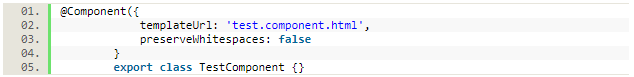
\includegraphics[width=1\columnwidth]{img/ng5_diff.png}
  \caption{\label{fig:ng_diff} Príklad zákazu medzier na vrstve komponentu}
\end{figure}

Ak by sme potrebovali zakázať biele znaky na úrovni celej aplikácie, voľbu by sme 
aplikovali v \textit{tsconfig.json} súbore nasledovne:

\begin{figure}[ht]
  \centering
  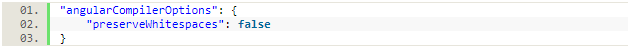
\includegraphics[width=1\columnwidth]{img/ng5_diff_2.png}
  \caption{\label{fig:ng_diff_2} Príklad zákazu medzier na aplikačnej vrstve}
\end{figure}

\begin{itemize}
\item Zvýšenie štandardizácie v prehliadačoch: 
v predchádzajúcich verziách Angular-u sme boli závislí na \textit{i18n} vždy, keď sme chceli podporiť
 internacionalizáciu v našej aplikácii. V aplikácii Angular 5 teraz nemusíme závisieť od \textit{i18n}.
 Poskytuje nové dátumové, číselné a menové potrubia, ktoré zvyšujú internacionalizáciu
 vo všetkých prehliadačoch a eliminujú potrebu \textit{i18n} polyfillov.
\item exportAs: 
v Angular 5 sa podporujú viacnásobné názvy pre direktívy aj komponenty.
\item HttpClient: 
pred verziou Angular 4.3 sa používal \textit{@angular/HTTP} modul pre všetky druhy požiadaviek \acrshort{http}. 
V Angular 5 bol tento modul nahradený novým modulom s názvom \textit{HttpClientModule}, ktorý 
sa nachádza pod balíkom \textit{@angular/common/http}.
\item Vylepšená podpora dekorátorov: 
v Angular 5 vieme použiť lambda výrazy namiesto menovania funkcií, ako tomu bolo predtým. 
V kóde vyzerá tento rozdiel napríklad nasledovne:
\end{itemize}

\begin{figure}[ht]
  \centering
  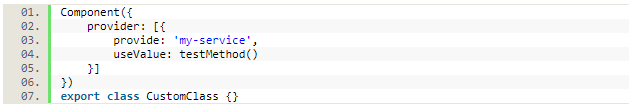
\includegraphics[width=1\columnwidth]{img/ng5_diff_3.png}
  \caption{\label{fig:ng_diff_3} Menovanie funkcie v skorších verziách Angularu}
\end{figure}

\begin{figure}[ht]
  \centering
  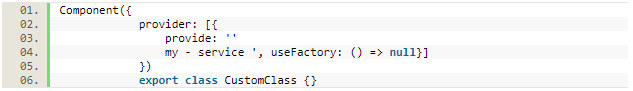
\includegraphics[width=1\columnwidth]{img/ng5_diff_4.png}
  \caption{\label{fig:ng_diff_4} Použitie lambda výrazu v Angular 5}
\end{figure}

\newpage
\begin{itemize}
\item Nové udalosti životného cyklu smerovača: 
v Angular 5 sa do smerovača pridalo niekoľko nových udalostí životného cyklu, ako sú 
\textit{ActivationStart, ActivationEnd,  ChildActivationStart, ChildActivationEnd, GuardsCheckStart, 
GuardsCheckEnd, ResolveStart and ResolveEnd}.
\item Angular 5 podporuje TypeScript vo verzii 2.3.
\item Vylepšenie rýchlosti kompilátora: 
zlepšenie v kompilátore umožnilo rýchlejšie vývojové buildovanie. Teraz môžeme 
jednoducho spustiť príkaz \textit{ng serve/s --aot } vo vývojovom príkazovom riadku 
a urýchliť buildovanie.
\end{itemize}

%------------------------------------------------------------------------------------------------------------------------
\subsubsection{RxJS - Observable}
\label{subsubsec:rxjs}

Reactive Extensions (Rx)\footnote{\url{http://reactivex.io/rxjs/}} je knižnica pre vytváranie
asynchrónnych programov a programov založených na udalostiach pomocou sledovateľných
sekvencií a operátorov dopytu v štýle \acrshort{linq}.

Dátové sekvencie môžu mať mnoho foriem, ako napríklad tok dát zo súboru 
alebo webovej služby, požiadavky na webové služby, systémové upozornenia
alebo sériu udalostí, ako je napríklad vstup pre používateľa.

Kód, ktorý sa zaoberá viacerými udalosťami alebo asynchrónnym výpočtom, sa rýchlo komplikuje,
pretože potrebuje vybudovať stavový stroj na riešenie problémov s objednávaním požiadaviek. 
Okrem toho sa kód musí zaoberať úspešným a neúspešným ukončením každého samostatného výpočtu. 
To vedie ku kódu, ktorý nedodržuje normálny tok riadenia, ktorý je mohutný a je náročné ho pochopiť
a ťažko sa udržiava.

Reaktívne rozšírenia reprezentujú všetky tieto dátové sekvencie ako pozorovateľné
sekvencie. Aplikácia sa môže prihlásiť k týmto pozorovateľným sekvenciám a prijímať
asynchrónne upozornenia pri príchode nových údajov.

\acrshort{rxjs} sa používa na rozvrhovanie asynchrónnych výpočtov a výpočtov založených na udalostiach.
V nástroji Rx sa \textit{observer} prihlási k \textit{Observable}. Potom \textit{observer} reaguje na akúkoľvek 
položku alebo sekvenciu položiek, ktoré \textit{Observable} vysiela. Tento vzor uľahčuje súbežné 
operácie, pretože sa nemusia blokovať počas čakania, kým \textit{Observable} nevyšle objekty.
Namiesto toho vytvoria strážcu vo forme \textit{observer-a}, ktorý je pripravený primerane 
reagovať na čokoľvek v budúcnosti, čo \textit{Observable} urobí.

\acrshort{rxjs} nemá žiadne závislosti a hladko spolupracuje s oboma
synchrónnymi dátovými tokmi, ako sú iteračné objekty v jazyku \acrlong{js} aj asynchrónnymi
tokmi s jedinou hodnotou, ako napríklad \textit{Promises}. \cite{rxjs}

Tabuľka \ref{table:2} referuje prehľad prístupov spracovania toku dát:
 
\begin{table}[h!]
\centering
\begin{tabular}{| c || c | c |} 
 \hline
& Jedna návratová hodnota & Viac návratových hodnôt \\ [0.5ex] 
\hline\hline
Synchronous/Interactive & Object & Iterables (Array|Set|Map|Obj)\\ 
\hline
Asynchronous/Reactive & Promise & Observable \\ 
\hline
\end{tabular}
\caption{Prehľad prístupov spracovania toku dát \cite{rxjs}}
\label{table:2}
\end{table}

%------------------------------------------------------------------------------------------------------------------------
\subsubsection{SCSS}
\label{subsubsec:scss}

\acrshort{sass}\footnote{\url{https://sass-lang.com/}} je preprocesor skriptovací jazyk, ktorý je interpretovaný alebo kompilovaný do
kaskádových štýlov (\acrshort{css}). SassScript je samotný skriptovací jazyk a pozostáva z dvoch syntaxí.
Pôvodná syntax, nazývaná ``odsadená syntax'', používa odsadenie na oddelenie kódových blokov
a nové riadky na oddelenie pravidiel. Používa zložené zátvorky na označenie blokov kódu
a bodkočiarky na oddelenie riadkov v rámci bloku. Nezáleží na úrovniach odsadenia alebo na
vynechanom priestore \cite{sass}. V skutočnosti je SCSS syntax nadradenou \acrshort{css} čo znamená, že SCSS
obsahuje všetky funkcie \acrshort{css}, ale navyše bola rozšírená o funkcie \acrshort{sass}-u. Súborom s odsadenou
syntaxou a SCSS sa tradične dávajú koncovky \textit{.sass}, respektíve \textit{.scss}. 

%------------------------------------------------------------------------------------------------------------------------
%------------------------------------------------------------------------------------------------------------------------
\subsection{Vývojové prostredie}
\label{subsec:develop_env}

Vyvíjali sme pod \acrshort{os} Ubuntu 16.04 LTS a ako integrované vývojové prostredie
sme použili editor Visual Studio Code. Tak ako pri predchádzajúcom projekte sme ako databázu
použili PostgreSQL, no aktualizovali sme ju na najnovšiu verziu 10.1.
Na vytvorenie virtuálneho prostredia sme použili pyenv\footnote{\url{https://github.com/pyenv/pyenv}}
a na inštaláciu potrebných balíčkov pre Python nástroj pip\footnote{\url{https://pypi.org/project/pip/}}.
%------------------------------------------------------------------------------------------------------------------------
%------------------------------------------------------------------------------------------------------------------------
\section{Implementácia}
\label{sec:implementation}

V danej kapitole popisujeme spôsob a postup pri vývoji používateľského rozhrania nášho rozvrhového
systému. Detailnejšie sa venujeme jednotlivým modulom aplikácie a ich implementácii ako samostatných
oddielov systému, z ktorých každý plní inú funkcionalitu a slúži na iné účely. Systému sme z predchádzajúcej
verzie ponechali rovnaký názov Elisa.

%------------------------------------------------------------------------------------------------------------------------
%------------------------------------------------------------------------------------------------------------------------
\subsection{Architektúra klienta}
\label{subsec:client_architecture}

Systém sme na strane webového klienta implementovali ako \acrshort{spa} (z angl. Single page application)
jednostránkovú aplikáciu . Pre tento typ aplikácií je príznačné, že sa jej zdrojové
kódy (\acrshort{html}, \acrshort{js} a \acrshort{css}) načítavajú už pri prvotnom
načítaní aplikácie. Stránkovanie je vykonávané prostredníctvom \textit{routing navigation},
kedy sa síce \acrshort{url} mení, ale stránka nemá potrebu sa počas behu obnovovať.
Na pohľad to teda vyzerá, že klikom na iný modul sa zobrazuje iná stránka, avšak v skutočnosti
sa na danej stránke mení iba jej obsah a nie stránka celá. 

%------------------------------------------------------------------------------------------------------------------------
%------------------------------------------------------------------------------------------------------------------------
\subsection{Štruktúra klienta}
\label{subsec:client_structure}

Klientskú časť našej aplikácie sme vyvíjali hierarchicky ako moduly, podmoduly a komponenty.
Najskôr sme ako prvé implementovali menšie časti - komponenty, ktoré sme neskôr spájali do
väčších podmodulov a nakoniec tie do ucelených modulových častí. Každý komponent má zadefinované
svoje vlastné správanie a zobrazovaciu šablónu. Jednotlivé moduly sú rozdelené ako podstránky aplikácie
a majú svoju \acrshort{url}, napríklad zobrazenie prehľadu má cestu \texttt{/dashboard}

Existuje osem hlavných blokov aplikácie Angular:
\begin{itemize}
\item Modul: Angular aplikácie sú modulárne a Angular má vlastný modulárny systém
nazvaný \textit{NgModules}. Modul je navrhnutý tak, aby vykonával jediný úkon.
\item Komponent: trieda so šablónou, ktorá sa zaoberá zobrazením (z angl. View) aplikácie
a obsahuje základnú logiku stránky.
\item Šablóny: forma \acrshort{html}, ktorá Angular-u  hovorí, ako má vykresliť
komponent. Zobrazenie je definované pomocou šablóny.
\item Metadáta: hovoria o tom, ako spracovať triedu (z angl. Class).
\item Väzba údajov: mechanizmus na koordináciu medzi časťami šablóny a
časťami komponentu. Existujú štyri formy syntaxe väzby údajov.
\item Direktívy: trieda s metadátami. Keď Angular vykresľuje šablóny,
transformuje \acrshort{dom} podľa pokynov uvedených v direktívach.
\item Služby: široká kategória zahŕňajúca akúkoľvek hodnotu, funkciu alebo
funkcionalitu, ktorú aplikácia potrebuje. Je to trieda s úzkym, ale dobre definovaným
účelom.
\item Vkladanie závislostí: spôsob, ako dodať novú inštanciu triedy s plne vytvorenými
závislosťami, ktoré vyžaduje. Väčšina závislostí sú služby. Angular toto vkladanie
používa na poskytovanie nových komponentov s potrebnými službami.
\end{itemize}

Naledujúci obrázok popisuje vnútornú architektúru použitú v Angular-e:
\begin{figure}[ht]
  \centering
  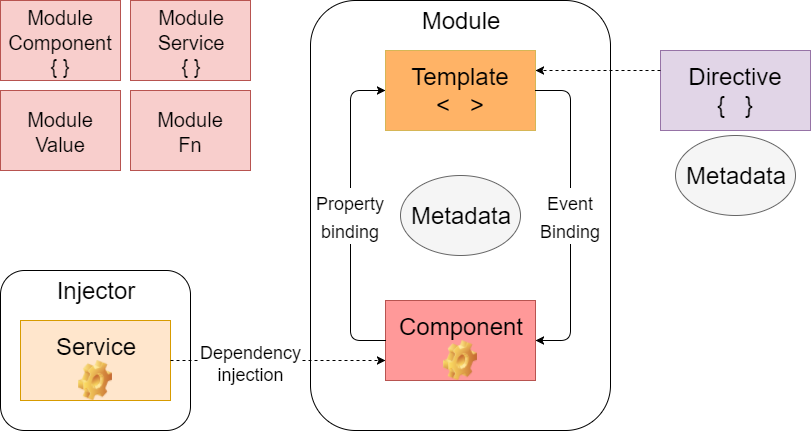
\includegraphics[width=0.8\columnwidth]{img/architecture_ang.png}
  \caption{\label{fig:architecture_ang} Architektúra použitá v Angular-e \cite{angular}}
\end{figure}

Pri implementácii sme postupovali najmä vo vývoji do šírky, čiže sme sa snažili o poskytnutie
minimálnej funkcionality s dôrazom na celkový dizajn a náhľad možných budúcich potrieb takejto
rozvrhovej aplikácie. Nedbali sme pritom len na potreby samotného rozvrhára, ale implementovali
sme aj moduly, ktoré môžu byť využívané inými použivateľmi, ktorí sa priamo nezúčastňujú 
rozvrhovania, ale systém má byť určený aj im. Jednotlivé komponenty sme sa snažili implementovať
tak, aby ich bolo možné kedykoľvek a kdekoľvek v aplikácii jednoducho opakovane použiť.

Medzi takéto komponenty patria:

\begin{itemize}
\item komponent registrácie a prihlasovania,
\item formulárové prvky a ich validácia,
\item prehľadové karty s informáciami o najdôležitejších metrikách,
\item prehľad blížiacich sa stretnutí a udalostí,
\item kalendár udalostí z viacerých časových náhľadov s funkcionalitou Drag\&Drop
a rozširovania ťahaním okrajov,
\item mailbox na mailovú komunikáciu,
\item chat na rýchlu konverzáciu,
\item zoznam kontaktov,
\item osobný profil používateľa,
\item konfiguračný panel,
\item horné menu a bočná navigácia,
\item smerovanie medzi stránkami aplikácie,
\item dialógové okná,
\item dizajnové prvky aplikácie.
\end{itemize}

Komponenty vytvárame pomocou Angular \acrshort{cli}. Príkazom \texttt{ng generate} vytvoríme komponent,
pridáme ho do deklarácií v našom \textit{ElisaModule}, ktorý sa následne importuje ako celok do
\textit{AppModule} na najvyššej vrstve aplikácie. \textit{ElisaModule} vlastne takýmto spôsobom importuje všetky
vytvorené hlavné komponenty a združuje ich na jednom mieste.
Vo všeobecnosti sa jednoduchý komponent vytvára nasledovne:

 \texttt{ng generate component  \textit{component\char`_name}}

Každý komponent má životný cyklus vytvorenia, aktualizácie a zničenia.
Spolu so súborom \textit{.ts} komponentu sa vytvorí trieda, ktorá implementuje \textit{OnInit} rozhranie z \textit{Core} knižnice.
Niektoré komponenty potrebujú vykonať volanie \acrshort{api} na načítanie údajov, ale komponent by to sám
o sebe nikdy nemal robiť. Na tieto účely sú v Angular používané súbory \textit{service}, takže sa
komponent môže sústrediť iba na zobrazovanie údajov a prenos údajov do iných komponentov,
ktoré ich potrebujú. V našom prípade pre komponent kalendár vyzerá úvodné načítanie dát nasledovne:

\newpage
\begin{figure}[ht]
  \centering
  \includegraphics[width=1\columnwidth]{img/code/getEvents_calendar.png}
  \caption{\label{fig:getEvents_calendar} Ukážka kódu inicialižačného načítania dát}
\end{figure}

V \textit{ngOnInit} časti uskutočníme požiadavku \acrshort{api} volania na aktualizovanie údajov
počas \textit{OnInit} fázy komponentu pri obnovení stránky, avšak prevedenie tohto \acrshort{api}
volania sa implementuje v \textit{service} súbore.

\begin{figure}[ht]
  \centering
  \includegraphics[width=1\columnwidth]{img/code/ngOnInit_calendar_2.png}
  \caption{\label{fig:ngOnInit_calendar_2} Ukážka kódu požiadavky v \textit{ngOnInit}}
\end{figure}

Takýto \textit{service} súbor môžme takisto vytvoriť pomocou Angular \acrshort{cli} nasledovne:

 \texttt{ng generate service \textit{service\char`_name} --module=\textit{module\char`_name}}

To vytvorí triedu \textit{service\char`_name} a pridá túto triedu služby medzi \textit{providers}
do \textit{module\char`_name} modulu.

Angular používa triedu \textit{HttpClient} na komunikáciu so vzdialeným serverom. Na použitie 
v našej službe (a kdekoľvek inde v aplikácii), musíme importovať \textit{HttpClientModule}
do \textit{AppModule}. Potom môžme vložiť \textit{HttpClient} do konštruktora nášho \textit{service} súboru.
Následne vytvoríme metódy na \acrshort{crud} operácie s dátami, ktoré volajú \acrshort{http} volania na \acrshort{api}.
Prihlásili sme sa k vrátenej \textit{Observable} a priradili vrátene dáta k deklarovanej premennej.

\newpage
\begin{figure}[ht]
  \centering
  \includegraphics[width=1\columnwidth]{img/code/service_calendar.png}
  \caption{\label{fig:service_calendar} Ukážka kódu metód v \textit{service} súbore}
\end{figure}

%------------------------------------------------------------------------------------------------------------------------
%------------------------------------------------------------------------------------------------------------------------
\subsection{Prehľad modulov aplikácie}
\label{subsec:modules_structure}

Tak ako sme už niekoľkokrát vyššie spomenuli, naša aplikácia je založená na moduloch, ktoré ako ucelené
časti kódu vykonávajú každý svoju špecifickú úlohu. V danej kapitole si popíšeme jednotlivé moduly
a priblížime si implementáciu niektorých dôležitejších komponentov a funkcionalít.

%------------------------------------------------------------------------------------------------------------------------
\subsubsection{Modul autentifikácie}
\label{subsubsec: authentication_module}

Tento modul aplikácie slúži na autentifikačné činnosti ako sú registrácia nového
a prihlásenie existujúceho používateľa. Do tohto modulu môže takisto patriť aj
stránka na obnovu zabudnutého hesla, stránka na zablokovanie konta v prípade
opakovaného chybného pokusu o prihlásenie prípadne stránka na potvrdenie
odoslania nového vygenerovaného hesla.

V prípade týchto komponentov na registráciu a prihlasovanie sme vytvorili formuláre
a potrebné polia na zadávanie vstupu pomocou Angular Material komponentov.
Na jednotlivé vyžadované polia sme aplikovali validátory (z angl. validators) 
a prostredníctvom \textit{Observable} počúvame na zmeny (\textit{valueChanges})
vykonávané na formuláry. Tieto polia sa teda validujú dynamicky a v prípadne nevalidnosti
je používateľ upozornený na porušené pravidlá, ktoré nedodržal počas zadávania vstupu.

\newpage
\begin{figure}[ht]
  \centering
  \includegraphics[width=1\columnwidth]{img/code/auth_forms.png}
  \caption{\label{fig:/auth_forms} Ukážka kódu na zavedenie validátorov a počúvania na zmeny}
\end{figure}

%------------------------------------------------------------------------------------------------------------------------
\subsubsection{Modul prehľad}
\label{subsubsec:dashboard_module}

Modul prehľad slúži ako hlavná stránka aplikácie. V nej sa používateľovi zobrazujú základné
informácie a metriky, ktoré sú pre neho podstatné, resp. by ho mohli zaujímať. Tieto metriky
je v budúcnosti možné meniť v závislosti od typu prihláseného používateľa na základe
používateľských práv, potrieb a preferencií.

K daným zobrazovaným informáciam a metrikám sú samozrejme potrebné dáta. Na takéto účely
sme si na klientovi vytvorili simulovanú databázu \textit{elisa-fake-db.service.ts}, ktorá nám
``vytvára'' potrebné dáta. Následne tieto dáta doťahujeme na našich Angular Material
\textit{widgetoch}. Ako návratové hodnoty pri získavaní dát používame \textit{Promise}, nakoľko
sa jedná o jednu návratovú hodnotu a nie celý tok (z angl. stream).

\begin{figure}[ht]
  \centering
  \includegraphics[width=1\columnwidth]{img/code/dashboard_promise.png}
  \caption{\label{fig:dashboard_promise} Ukážka kódu na doťahovanie dát pomocou \textit{Promise}}
\end{figure}
\newpage
%------------------------------------------------------------------------------------------------------------------------
\subsubsection{Modul rozvrhovanie}
\label{subsubsec:scheduling_module}

Modul rozvrhovanie slúži na prácu s rozvrhmi a kalendárom udalostí. Tento modul
je základným stavebným kameňom pre používateľa typu rozvrhár. Medzi základné
možnosti tohto modulu patrí predovšetkým vkladanie nových udalostí do kalendára,
upravovanie a mazanie existujúcich udalostí,
funkcionalita Drag\&Drop na zmenu časového umiestnenia udalosti v rozvrhu
a funkcionalita rozširovania časovej rezervácie udalosti ťahaním jej okrajov.

\newpage
\begin{figure}[ht]
  \centering
  \includegraphics[width=1\columnwidth]{img/screens/add.png}
  \caption{\label{fig:add} Komponent pridávania udalosti do kalendára}
\end{figure}

\begin{figure}[ht]
  \centering
  \includegraphics[width=1\columnwidth]{img/code/calendar_json_examlpe.png}
  \caption{\label{fig:calendar_json_examlpe} Ukážka úryvku JSON objektu dát kalendára}
\end{figure}
\newpage

\begin{figure}[ht]
  \centering
  \includegraphics[width=1\columnwidth]{img/code/calendar_drag.png}
  \caption{\label{fig:calendar_drag} Ukážka kódu implementácie funkcionality Drag\&Drop}
\end{figure}

\begin{figure}[ht]
  \centering
  \includegraphics[width=1\columnwidth]{img/code/calendar_resize.png}
  \caption{\label{fig:calendar_resize} Ukážka kódu implementácie funkcionality ``ťahanie okrajov''}
\end{figure}

Funkcionality súvisiace s kalendárom sme implementovali za pomoci komponentov a nástrojov
angular-calendar\footnote{\url{https://github.com/mattlewis92/angular-calendar}}.

%------------------------------------------------------------------------------------------------------------------------
\subsubsection{Modul komunikácia}
\label{subsubsec:communication_module}

Tento modul zabezpečuje komunikačný kanál systému. V budúcnosti bude možné
tento mailový klient napojiť na správy z AIS. Okrem komponentu mailovej komunikácie
tento modul obsahuje aj komponent chat-u, ktorý má slúžiť predovšetkým na rýchlu
komunikáciu medzi používateľmi. Posledným komponentom komunikačného modulu
je zoznam kontaktov na prezeranie. Implementovali sme množstvo okrajových
funkcionalít na manipuláciu s mailami a správami, ich vyberanie, označovanie atď.
Dáta v podobe správ a kontaktov sme taktiež doťahovali z našej simulovanej databázy. 

%------------------------------------------------------------------------------------------------------------------------
\subsubsection{Modul profil}
\label{subsubsec:profile_module}

Modul profilu zobrazuje najzákladnejšie informácie o prihlásenom používateľovi. V budúcnosti
tu vzniká možnosť rozšírenia na zobrazovanie profilov aj iných používateľov, napríklad po kliknutí
na niektorý kontakt v zozname prihláseného používateľa prípadne po celkovom vyhľadávaní
osôb v systéme. Tento modul má zatiaľ iba čisto informatívny charakter o používateľových osobných údajoch.
%------------------------------------------------------------------------------------------------------------------------
%------------------------------------------------------------------------------------------------------------------------
\subsection{Dizajn a konfigurácia používateľského rozhrania}
\label{subsec:app_gui_design}

Dizajn používateľského rozhrania sme sa snažili orientovať podľa moderných trendov
vývoja webových aplikácií. Kaskádové štýly \textit{scss} sme aplikovali na globálnej úrovni
a pre niektoré komponenty so špeciálnymi potrebami sme vytvárali lokálne \textit{scss}
súbory.

\begin{figure}[ht]
  \centering
  \includegraphics[width=1\columnwidth]{img/screens/create_schedule.png}
  \caption{\label{fig:create_schedule} Dizajn používateľského rozhrania kalendára udalostí}
\end{figure}

Celá aplikácia je responzívna, to znamená, že je schopná sa prispôsobovať rôznym
rozlíšeniam zariadení pri zachovaní plnej funkcionality aplikácie. To v budúcnosti eliminuje potrebu
vyvíjania dodatočnej mobilnej aplikácie. Responzívnosť používateľského rozhrania sme zabezpečili
pomocou externých direktív vytvorených v nástroji Angular Flex-Layout\footnote{\url{https://github.com/angular/flex-layout}}.

\newpage
\begin{figure}[ht]
  \centering
  \includegraphics[width=1\columnwidth]{img/code/responsive_fxlayout.png}
  \caption{\label{fig:responsive_fxlayout} Ukážka použitia direktív pre zachovanie responzívnosti komponentu}
\end{figure}

Jednou z funkcionalít, ktorú naša aplikácia poskytuje, je možnosť konfigurácie zobrazovania
elementov v používateľskom rozhraní. Používateľ si môže napríklad zmeniť rozloženie navigačných panelov,
vie si určiť, či majú byť dané panely roztiahnuté alebo skryté, môže si prispôsobovať farebné prevedenie
panelov podľa svojich potrieb a preferencií, prípadne si vie meniť zobrazenie aplikácie na zúžené alebo v plnom rozlíšení. 

\begin{figure}[ht]
  \centering
  \includegraphics[width=1\columnwidth]{img/screens/customize.png}
  \caption{\label{fig:customize} Príklad vlastnej konfigurácie používateľského rozhrania}
\end{figure}



